\documentclass[letterpaper]{article}

\usepackage[parfill]{parskip}
\usepackage[margin=1in]{geometry}
\usepackage{tocstyle}
\setcounter{tocdepth}{5}
\setcounter{secnumdepth}{5}
\renewcommand*\thesection{\arabic{section}.0 }
\renewcommand*\thesubsection{\arabic{section}.\arabic{subsection}}
\usepackage{sectsty}
\usepackage{graphicx}
\sectionfont{\LARGE}

\usepackage{lastpage}
\makeatletter
\renewcommand{\@oddfoot}{\hfil \thepage/\pageref{LastPage} \hfil}
\makeatother

\begin{document}
\begin{center}
	\LARGE{A guide to data visualization using BL.plotting.general}\\~\\
	\large{Christine P'ng \& Jeff Green}\\~\\
	\large{\today}
\end{center}
\tableofcontents

\newpage
\section{Introduction}
Why does data visualization even matter? After all, data visualization takes work. Datasets are often complex, having millions of data points and many dimensions. Decisions have to be made regarding the best way of highlighting the main message. Aesthetic considerations require knowledge of colour theory, typography, composition, and more. Why do people go through all the trouble?

The reason is that it is often faster and easier for a person to process data visually. Noticing relationships between data points in a spreadsheet requires much more careful attention compared to viewing the same data points in a chart. Graphs can be used to first find trends in the data, and later to illustrate and highlight messages in data for communication to others \cite{Anscombe}\cite{wong-dataexploration}.

\subsection{Stages of figure creation}
When it comes to making figures, there are four main steps:
\begin{enumerate}
\item Understand the data and know what the plot is supposed to convey
\item Determine which chart-type is best suited to the data
\item Design the figure to communicate clearly and be aesthetically pleasing
\item Evaluate if other people can understand it
\end{enumerate}

Understanding a dataset is especially important when a dataset is large and not all of it is relevant for plotting. For example, if a dataset has five dimensions, but only two are relevant to convey the main message, it could be appropriate to only display the relevant dimensions. In addition, knowing what the data is trying to convey is helpful for choosing the correct chart-type and properly emphasizing the data. 

\begin{figure}[!ht]
  \begin{center}
     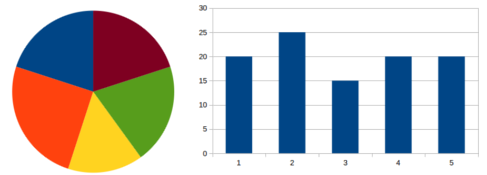
\includegraphics[width=80mm]{Figures/pie_vs_bar_chart.png}
     \caption{Pie chart and barplot displaying identical data}
  \end{center}
\end{figure}

Different chart-types are suited for different data-types, and emphasize different kinds of relationships. Using the correct chart-type will improve the readability of the data. It is important to note that some methods of visually encoding data are easier to interpret than others (Table 1). For example, pie charts are difficult to interpret because people struggle to translate angles and areas into exact numerical values. The difference between a 25\% slice and a 20\% slice is not easy to distinguish. Instead, a barchart which compares lengths on a common scale would be easier to read. Display methods which are more accurately interpreted should be selected over methods which are relatively difficult to accurately interpret \cite{wong1}\cite{cleveland}. 

\begin{table}
\begin{center}
\begin{tabular}{ l  l }
\hline
Rank & Aspect judged\\
\hline
1 & Position along a common scale\\
2 & Position on identical but nonaligned scales\\
3 & Length \\
4 & Angle, Slope\\
5 & Area\\
6 & Volume, Density, Colour saturation\\
7 & Colour hue\\
\end{tabular}
\end{center}
\caption{Tasks ordered from most to least accurate. Adapted from Cleveland \& McGill.}
\end{table}

Figures should be designed to enhance a viewer's ability to compare data and draw appropriate conclusions \cite{tufte}. This can be done through careful arrangement of a figure, such as placing related elements near each other, highlighting important items, selecting appropriate colours and fonts, and more. Poorly-designed figures can distort the truth and lead viewers to draw inaccurate conclusions \cite{tufte}. 

To check if a figure is effective, it is helpful to request an interpretation of the figure from someone who does not know what the intended message is. This test (often conducted multiple times) can reveal how clear a figure is.

\subsection{What is BL.plotting.general?}
BL.plotting.general is a software package for generating publication-quality, customizable plots. It produces a variety of chart-types, ranging from common charts for simple datasets to novel charts for displaying highly-dimensional datasets.

This package is built on top of the \texttt{lattice} package \cite{lattice}, which is an implementation of Trellis graphics for R. Therefore, when plots are created in this package, parameters are passed to the appropriate \texttt{lattice} function and a Trellis object is created. 

\section{Plotting Functions}
The following  chart-types available in BL.plotting.general:

\begin{center}
\begin{tabular}{l  l  l}
\hline
Chart-type & Data displayed & Encoding method\\
\hline
Barplot & Counts or proportions & Length\\
Boxplot & Distributions (summary statistics) & Length, Position\\
Dendrogram & Clustering arrangement & Length, Position \\
Density plot & Distributions & Area \\
Dotmap & Matrix of data points & Area, Colour saturation, Colour hue \\
Heatmap & Matrix of data points (ex. gene expression) & Colour saturation, Colour hue \\
Hexbinplot & Comparison of two variables & Colour saturation, Colour hue \\
Histogram & Distribution (binned into ranges) & Area, Length \\
Manhattan plot & Significance of SNPs at genome locations & Position \\
Multiplot & (variety) & (variety) \\
Polygon plot & Time-series or iterative data & Area \\
Quantile-quantile plot & Comparison of distributions & Position \\
Scatterplot & Comparison of two variables & Position \\
Segplot & Distributions (summary statistics) & Position \\
Strip plot & Distributions & Position \\
Violin plot & Distributions (optional summary statistics) & Area, Length, Position \\
\end{tabular}
\end{center}
\bigskip
Each plotting function is designed to display different kinds of data, and to highlight different relationships in the data. 

\subsection{Scatterplot}
\begin{verbatim}
create.scatterplot
\end{verbatim}

The scatterplot compares two variables on a Cartesian coordinate grid by plotting individual data points. It can be used to investigate correlation between variables, and lines can join the points to emphasize trends. Error bars may be added to each point, and the create.scatterplot function can also determine optimal label positions for points. This versatile function is used to create other plot types, including receiver operating characteristic (ROC) curves.

An interesting note is that scatterplots appear more correlated when scales are increased. This means that when the points in a scatterplot use less of the total plotting space available, a stronger association is perceived compared to when the plotting space is filled \cite{cleveland-scatter}.

\subsubsection{Simple scatterplot}
The scatterplot function accepts data in the form of an R  data frame. Here is an example of a data frame created using the \verb|microarray| dataset provided with BL.plotting.general.
\begin{verbatim}
scatter.data <- data.frame(
    sample.one = microarray[1:800,1],
    sample.two = microarray[1:800,2]
    );
\end{verbatim}

A simple scatterplot has two requirements: the data frame, and a formula to indicate the x and y components of the data frame. In this example a file name is also included so that the plot will be saved to file.
\begin{verbatim}
create.scatterplot(
    filename = "Scatterplot_Minimal_Input.png",
    formula = sample.two ~ sample.one,
    data = scatter.data
    );
\end{verbatim}
\begin{figure}[!ht]
  \begin{center}
     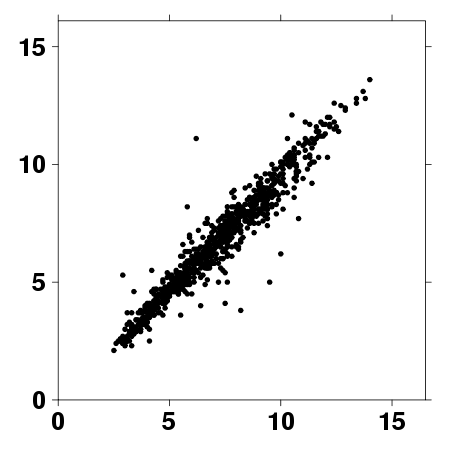
\includegraphics[width=50mm]{Figures/Scatterplot_Minimal_Input.png}
     \caption{Simple scatterplot}
  \end{center}
\end{figure}

\subsubsection{Scatterplot with formatted axes}
The scatterplot can be customized very easily by specifying the appropriate parameters. 
\begin{verbatim}
create.scatterplot(
    filename = "Scatterplot_Axes_Labels.png",
    formula = sample.two ~ sample.one,
    data = scatter.data,

    # This specifies the plot title
    main = "Axes & labels",
    
    # These specify the axes titles
    xlab.label = "Sample 1",
    ylab.label = "Sample 2",

    # These specify where axes tick marks appear
    xat = seq(0, 16, 2),
    yat = seq(0, 16, 2),
    
    # These specify the axes ranges
    xlimits = c(0, 15),
    ylimits = c(0, 15),
    
    # These specify the font sizes of the axes titles and tick mark labels
    xaxis.cex = 1,
    yaxis.cex = 1,
    xlab.cex = 1.5,
    ylab.cex = 1.5
    );
\end{verbatim}
\begin{figure}[!ht]
  \begin{center}
     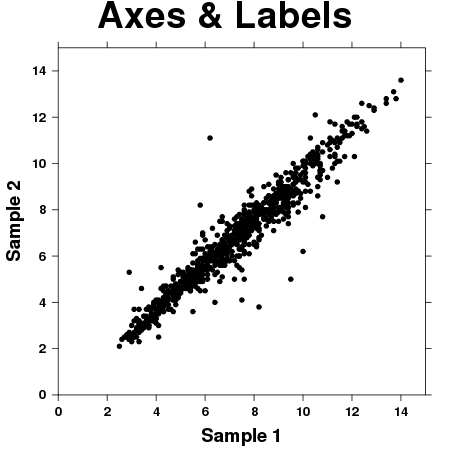
\includegraphics[width=50mm]{Figures/Scatterplot_Axes_Labels.png}
     \caption{Scatterplot with formatted axes}
  \end{center}
\end{figure}

\subsubsection{Scatterplot with gridlines}
Additional parameter changes will continue to customize the plot.
\begin{verbatim}
create.scatterplot(
    filename = "Scatterplot_Grid.png",
    formula = sample.two ~ sample.one,
    data = scatter.data,
    main = "Gridlines",
    xlab.label = "Sample 1",
    ylab.label = "Sample 2",
    xat = seq(0, 16, 2),
    yat = seq(0, 16, 2),
    xlimits = c(0, 15),
    ylimits = c(0, 15),
    xaxis.cex = 1,
    yaxis.cex = 1,
    xlab.cex = 1.5,
    ylab.cex = 1.5,
    
    # The type of plotting character used is changed using the "pch" parameter
    # Plotting characters with borders may accept both border colour and fill colour
    # The available options are found in the help files for "pch"
    pch = 21,
    col = "black",
    
    # Gridlines are created using the "type" parameter
    # Here, the "p" indicates points, and the "g" indicates grid
    # Other options for the "type" parameter are found in the "xyplot" documentation
    type = c("p", "g")
    );
\end{verbatim}
\begin{figure}[!ht]
  \begin{center}
     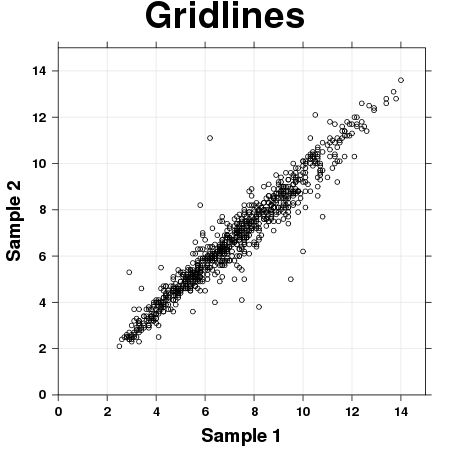
\includegraphics[width=50mm]{Figures/Scatterplot_Grid.png}
     \caption{Scatterplot with grid lines}
  \end{center}
\end{figure}

\subsubsection{Scatterplot with labelled points}
The scatterplot function is able to calculate optimal label positions for labelling individual points. 
\begin{verbatim}
# Determine which point(s) should get labels
max.one <- which(scatter.data$sample.one == max(scatter.data$sample.one));
max.one.x <- max(scatter.data$sample.one);
max.one.y <- scatter.data$sample.two[max.one];

create.scatterplot(
    filename = "Scatterplot_Point_Labels.png",
    formula = sample.two ~ sample.one,
    data = scatter.data,
    main = "Point labels",
    xlab.label = "Sample 1",
    ylab.label = "Sample 2",
    xat = seq(0, 16, 2),
    yat = seq(0, 16, 2),
    xlimits = c(0, 15),
    ylimits = c(0, 15),
    xaxis.cex = 1,
    yaxis.cex = 1,
    xlab.cex = 1.5,
    ylab.cex = 1.5,
    pch = 21,
    col = "black",
    fill = "transparent",
    type = c("p", "g"),
    
    # This allows for auto-placement of labels based on point locations
    # (otherwise given coordinates will be used)
    text.guess.labels = TRUE,
    
    # Here the labels and corresponding points are specified
    add.text = TRUE,
    text.x = max.one.x,
    text.y = max.one.y,
    text.labels = rownames(microarray)[max.one]
    );
\end{verbatim}
\begin{figure}[!ht]
  \begin{center}
     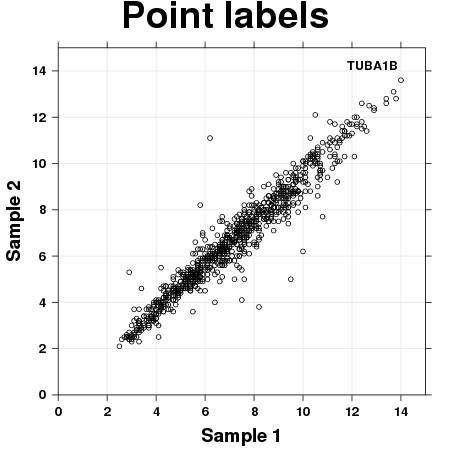
\includegraphics[width=50mm]{Figures/Scatterplot_Point_Labels.png}
     \caption{Scatterplot with point labelling}
  \end{center}
\end{figure}

\subsection{Boxplot}
\begin{verbatim}
create.boxplot
\end{verbatim}

The boxplot is used to display distributions of data. It is also known as the box-and-whisker plot. The `box' ranges from the first to the third quartile, showing the interquartile range. The line within the box indicates the median (not the mean), and whiskers have variable meaning, such as the maximum and minimum of the data (but they are not error bars; they are not the s.d. or s.e.m). The meaning of whiskers should be indicated, and outliers may be plotted as points \cite{Krzywinski}. BL.plotting.general defaults to setting the whiskers to the most extreme data point within 1.5 $\times$ IQR of the edge of the box.

\subsubsection{Simple boxplot}
The boxplot also requires a data frame and corresponding formula as its minimum input.
\begin{verbatim}
boxplot.data <- data.frame(
    x <- as.vector(t(microarray[1:10,1:58])),
    y <- as.factor(rep(rownames(microarray[1:10,1:58]), each = 58))
    );
    
create.boxplot(
    filename = "Boxplot_Minimal_Input.png",
    formula = y ~ x, 
    data = boxplot.data
    );
\end{verbatim}
\begin{figure}[!ht]
  \begin{center}
     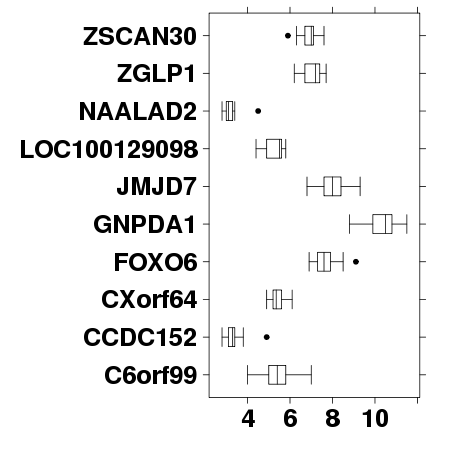
\includegraphics[width=50mm]{Figures/Boxplot_Minimal_Input.png}
     \caption{Simple boxplot}
  \end{center}
\end{figure}

\subsubsection{Boxplot with colour}
Customization of boxplot parameters is done by specifying the appropriate parameters.
\begin{verbatim}
create.boxplot(
    filename = "Boxplot_Colours.png",
    formula = y ~ x, 
    data = boxplot.data,

    # The colour of the boxes is specified by this parameter
    fill = default.colours(1)
    );
\end{verbatim}
\begin{figure}[!ht]
  \begin{center}
     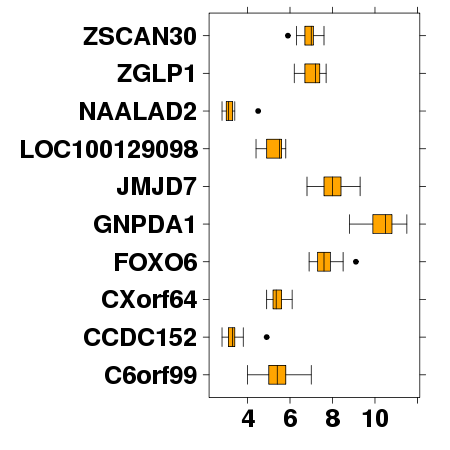
\includegraphics[width=50mm]{Figures/Boxplot_Colours.png}
     \caption{Boxplot with colour}
  \end{center}
\end{figure}

\subsubsection{Boxplot with background shading}
Coloured rectangles can be drawn in plots.

\begin{verbatim}
create.boxplot(
    filename = "Boxplot_Bg_Rect.png",
    formula = y ~ x, 
    data = boxplot.data,
    fill = default.colours(1),
	
    # This parameter must be specified for rectangles to be drawn
    add.rectangle = TRUE,
	
    # The coordinates of the rectangles are given by four parameters
    xleft.rectangle = 0,
    xright.rectangle = 13,
    ybottom.rectangle = seq(0.5, 8.5, 2),
    ytop.rectangle = seq(1.5, 9.5, 2),
	
    # The colour of the rectangles are given by this parameter
    col.rectangle = "grey",
	
    # The alpha of the rectangle is specified here
    alpha.rectangle = 0.25
    );
\end{verbatim}
\begin{figure}[!ht]
  \begin{center}
     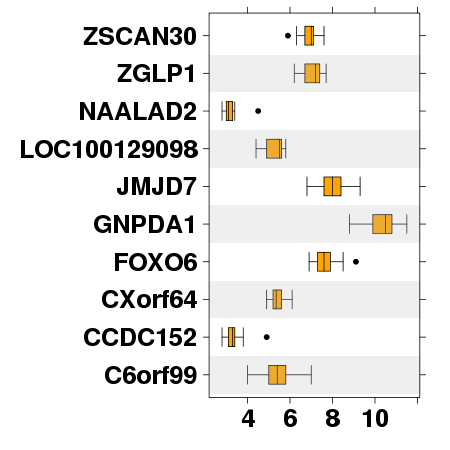
\includegraphics[width=50mm]{Figures/Boxplot_Bg_Rect.png}
     \caption{Boxplot with rectangles}
  \end{center}
\end{figure}

\subsubsection{Sorted boxplot}
To make comparisons clearer for viewers, the boxplots can be sorted by median value.

\begin{verbatim}
create.boxplot(
    filename = "Boxplot_Sorted.png",
    formula = y ~ x, 
    data = boxplot.data,
    fill = default.colours(1),
    add.rectangle = TRUE,
    xleft.rectangle = 0,
    xright.rectangle = 13,
    ybottom.rectangle = seq(0.5, 8.5, 2),
    ytop.rectangle = seq(1.5, 9.5, 2),
    col.rectangle = "grey",
    alpha.rectangle = 0.25,
    
    # this parameter can sort in either increasing or decreasing order
    sample.order = "increasing"
    );
\end{verbatim}
\begin{figure}[!ht]
  \begin{center}
     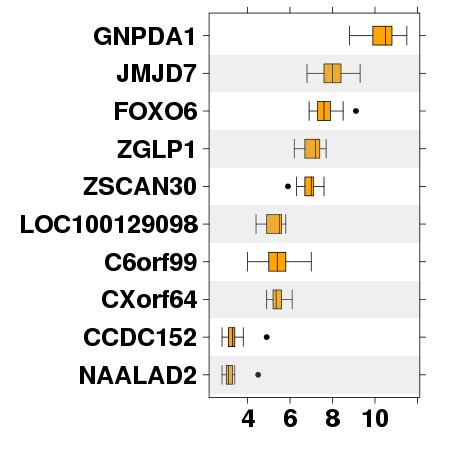
\includegraphics[width=50mm]{Figures/Boxplot_Sorted.png}
     \caption{Sorted boxplot}
  \end{center}
\end{figure}

\subsection{Heatmap}
\begin{verbatim}
create.heatmap
\end{verbatim}

The heatmap is a matrix with values represented by colour value and hue. It is often used to display gene expression levels compared against samples. One strength of the heatmap is that it is able to display many data points with more dimensions: it displays a matrix of values where each cell encodes a value through colour, and is associated with both an x-axis and y-axis value. 

However, colour is a subjective method of conveying data. It is useful for displaying general trends and comparing values, but is not accurate for conveying exact values. Neighbouring colours change the perception of a colour such that a particular colour surrounded by lighter colours will appear darker, and vice versa. This means that two cells in a heatmap which are the same colour can appear to be different colours because of the cells surrounding them \cite{wong2}. One option for minimizing this bias is by clustering the heatmap so that similar colours will neighbour each other. Another option is to add grid lines to help distinguish the neighbouring colours. 

\subsubsection{Simple heatmap}
The minimal input for a heatmap is either a data frame or matrix. 

\begin{verbatim}
create.heatmap(
    filename = "Heatmap_Minimal_Input.png",
    x = microarray[1:20, 1:20]
    );
\end{verbatim}

\begin{figure}[!ht]
  \begin{center}
     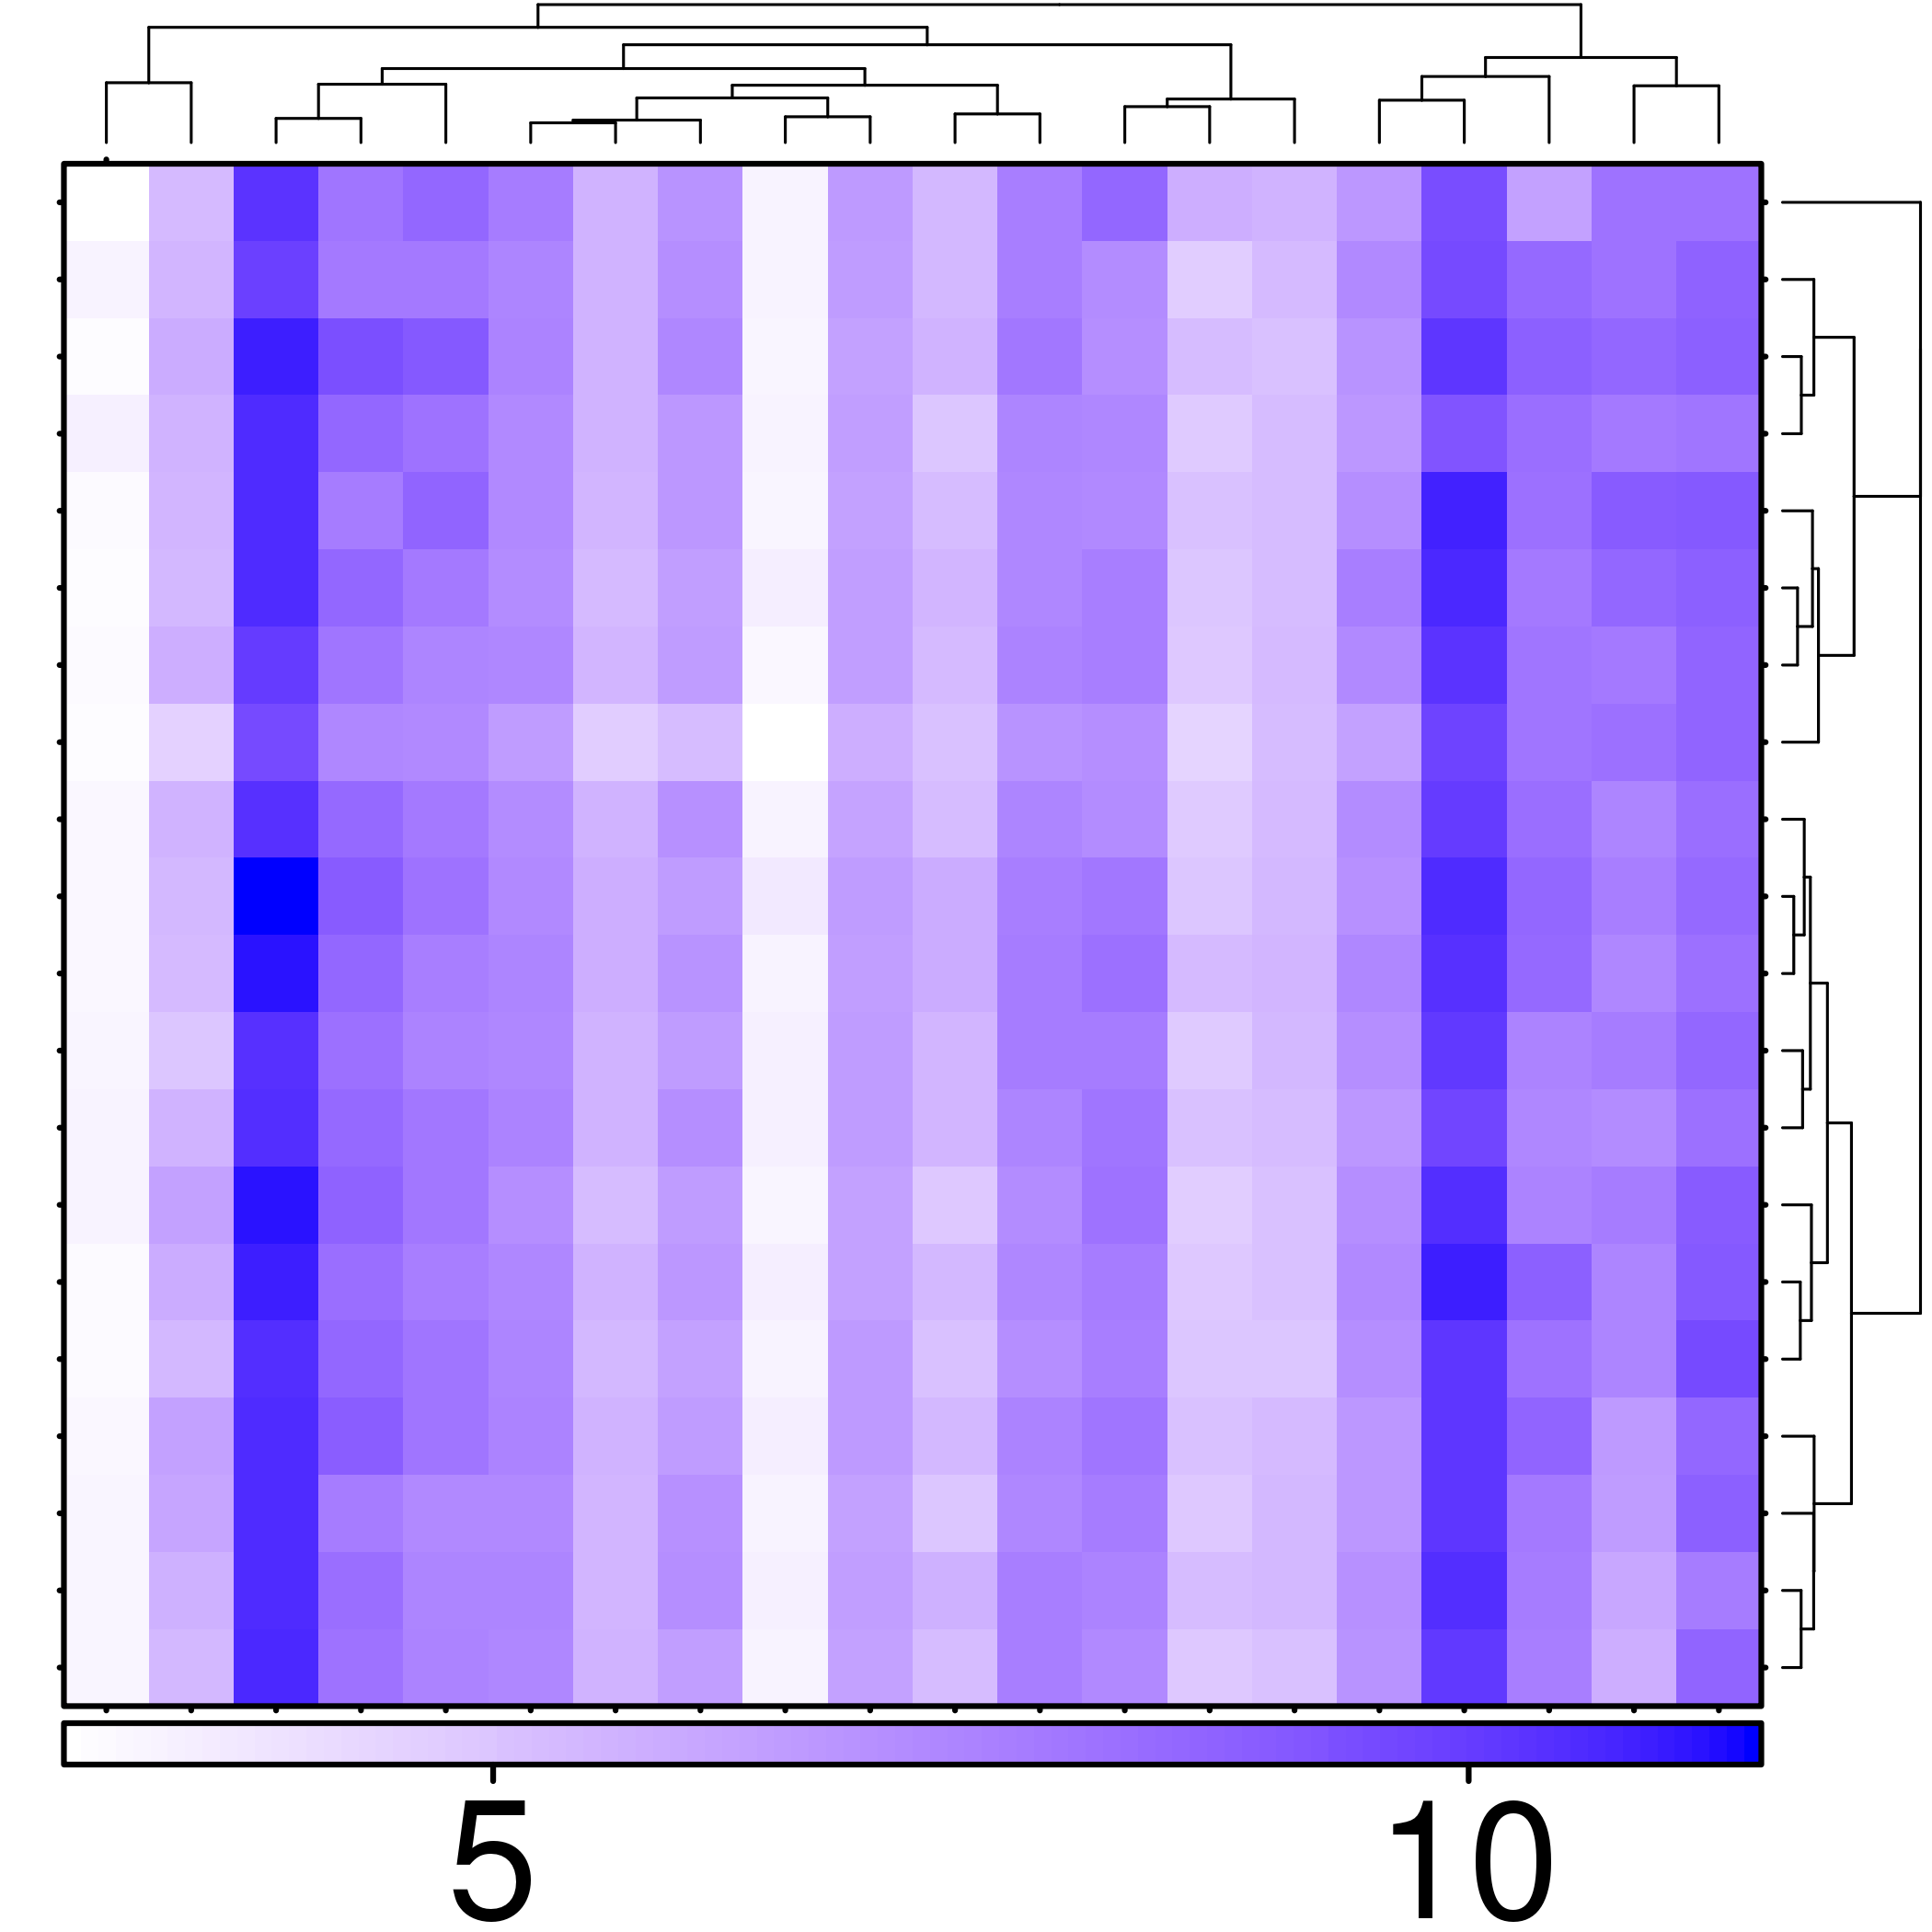
\includegraphics[width=50mm]{Figures/Heatmap_Minimal_Input.png}
     \caption{Simple heatmap}
  \end{center}
\end{figure}

\subsubsection{Heatmap with formatted axes}
Axes formatting can help the appearance of the plot. The heatmap function estimates an appropriate font size based on the size of the data set.
\begin{verbatim}
create.heatmap(
    filename = "Heatmap_Axes.png",
    x = microarray[1:20, 1:20],
    
    # Formatting the colour key
    colourkey.cex = 1,
    colourkey.labels.at = seq(2, 12, 1),    
    
    # Setting the labels to NA results in default labels
    xaxis.lab = NA,
    yaxis.lab = NA,
    
    # Setting the font style (default is bold, 1 is roman)
    xaxis.fontface = 1,
    yaxis.fontface = 1
    );
\end{verbatim}

\begin{figure}[!ht]
  \begin{center}
     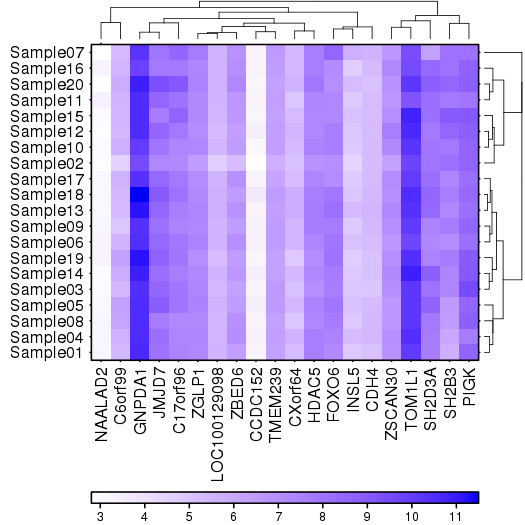
\includegraphics[width=50mm]{Figures/Heatmap_Axes.png}
     \caption{Heatmap with formatted axes}
  \end{center}
\end{figure}

\subsubsection{Heatmap with different clustering}
The heatmap defaults to clustering using the``diana" method (divisive analysis clustering). Other clustering options include all agglomerative clustering methods available in hclust.

\begin{verbatim}
create.heatmap(
    filename = "Heatmap_Clustering.png",
    x = microarray[1:20, 1:20],
    colourkey.cex = 1,
    colourkey.labels.at = seq(2, 12, 1),    
    xaxis.lab = NA,
    yaxis.lab = NA,
    xaxis.fontface = 1,
    yaxis.fontface = 1,
    
    # The clustering method used is specified here
    # If no clustering is desired, set this to "none"
    clustering.method = "complete",
    
    # The distance measure used can also be selected
    rows.distance.method = "euclidean",
    cols.distance.method = "manhattan"
    );
\end{verbatim}

\begin{figure}[!ht]
  \begin{center}
     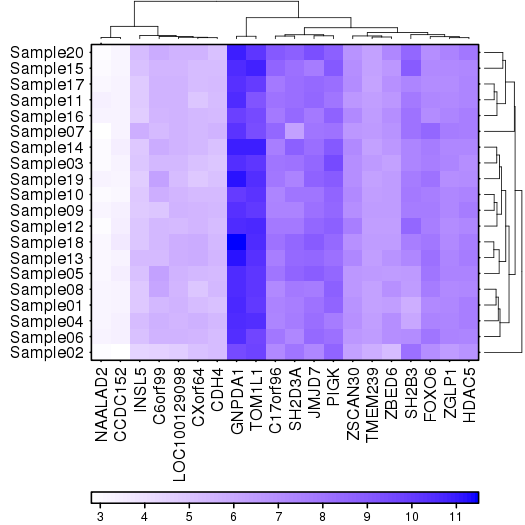
\includegraphics[width=50mm]{Figures/Heatmap_Clustering.png}
     \caption{Heatmap with different clustering}
  \end{center}
\end{figure}

\subsubsection{Heatmap with stratified clustering}
Heatmap clustering can be stratified so that segments of the data can be clustered separately.

\begin{verbatim}
create.heatmap(
    filename = "Heatmap_Stratified_Clustering.png",
    x = microarray[1:20, 1:20],
    colourkey.cex = 1,
    colourkey.labels.at = seq(2, 12, 1),    
    xaxis.lab = NA,
    yaxis.lab = NA,
    xaxis.fontface = 1,
    yaxis.fontface = 1,
    clustering.method = "complete",
    rows.distance.method = "euclidean",
    cols.distance.method = "manhattan",
 
    # Specify the groups. In this example clustering is done by columns
    stratified.clusters.cols = list(c(1:10), c(11:20)),
    
    # Adding line to show division between two strata
    grid.col = TRUE,
    col.lines = 10.5,
    col.lwd = 5,
    col.colour = "red"
    );
\end{verbatim}

\begin{figure}[!ht]
  \begin{center}
     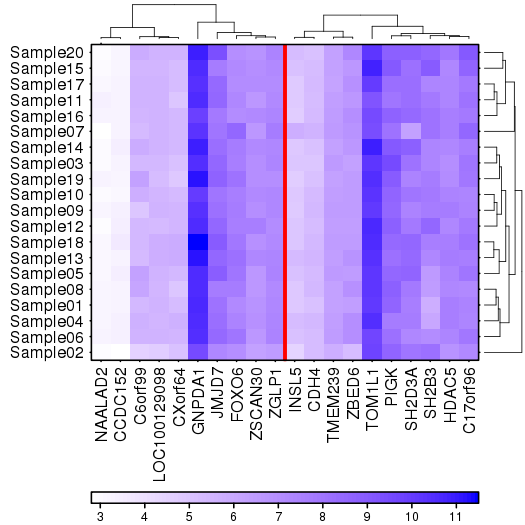
\includegraphics[width=50mm]{Figures/Heatmap_Stratified_Clustering.png}
     \caption{Heatmap with stratified clustering}
  \end{center}
\end{figure}

\subsubsection{Heatmap with covariates}
Covariate bars are often added to heatmaps to add additional information. In this example, the sex of each sample is indicated using a covariate bar.

\begin{verbatim}
# Creating a covariate bar to indicate sex
sample.covariate <- list(
    rect = list(
        col = "black",
        fill = force.colour.scheme(patient$sex[1:20], scheme = "sex"),
        lwd = 1.5
        )
    );

# Creating legend to match covariate bar
sample.cov.legend <- list(
    legend = list(
        colours =  force.colour.scheme(c("male",  "female"), scheme = "sex"),
        labels = c("male", "female"),
        title = "Sex"
        )
    );
    
create.heatmap(
    filename = "Heatmap_Covariates.png",
    x = microarray[1:20, 1:20],
    colourkey.cex = 1,
    colourkey.labels.at = seq(2, 12, 1),    
    xaxis.lab = NA,
    yaxis.lab = NA,
    xaxis.fontface = 1,
    yaxis.fontface = 1,

    # Adding covariates and corresponding legend
    covariates = sample.covariate,
    covariate.legend = sample.cov.legend
    );
\end{verbatim}

\begin{figure}[!ht]
  \begin{center}
     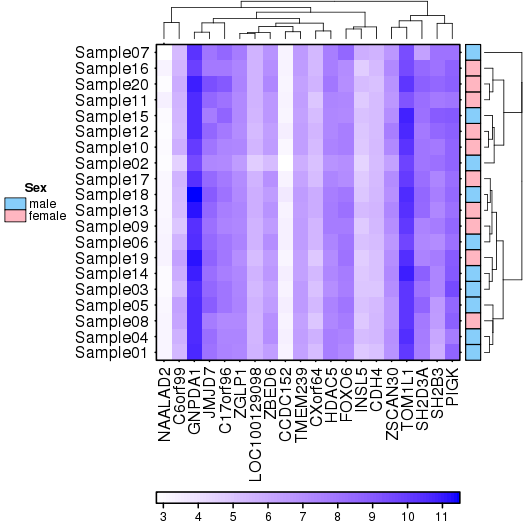
\includegraphics[width=50mm]{Figures/Heatmap_Covariates.png}
     \caption{Heatmap with covariates}
  \end{center}
\end{figure}

\subsubsection{Heatmap with grid lines}
Using grid lines can help to more accurately perceive the differences between colours.
\begin{verbatim}
create.heatmap(
    filename = "Heatmap_Gridlines.png",
    x = microarray[1:20, 1:20],
    colourkey.cex = 1,
    colourkey.labels.at = seq(2, 12, 1),    
    xaxis.lab = NA,
    yaxis.lab = NA,
    xaxis.fontface = 1,
    yaxis.fontface = 1,

    # Turning grid lines on
    grid.row = TRUE,
    grid.col = TRUE,
    
    # Setting the colour of the grid lines 
    row.colour = "white",
    col.colour = "white",
    
    # Setting the width of the grid lines
    row.lwd = 3,
    col.lwd = 3
    );
\end{verbatim}

\begin{figure}[!ht]
  \begin{center}
     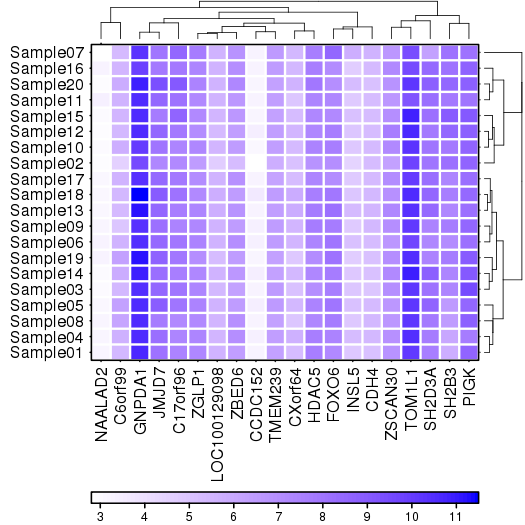
\includegraphics[width=50mm]{Figures/Heatmap_Gridlines.png}
     \caption{Heatmap with grid lines}
  \end{center}
\end{figure}


\subsubsection{Heatmap with discrete colours}
Sometimes heatmaps are used to display data with can be divided into discrete bins. In these cases, it is appropriate to use discrete colour schemes. The example below illustrates how a discrete colour scheme is created.

\begin{verbatim}
create.heatmap(
    filename = "Heatmap_Discrete.png",
    x = microarray[1:20, 1:20],
    colourkey.cex = 1,
    colourkey.labels.at = seq(2, 12, 1),    
    xaxis.lab = NA,
    yaxis.lab = NA,
    xaxis.fontface = 1,
    yaxis.fontface = 1,

   # Set the colour scheme
   # Setting more "total.colours" than colours  in "colour.scheme" creates a discretized gradient
   colour.scheme = default.colours(5, palette.type = "spiral.sunrise"),
   
   # Specify how many total colours (add one for a null colour)
   # In this example, 5 colours will be displayed
   total.colours = 6
   );
\end{verbatim}

\begin{figure}[!ht]
  \begin{center}
     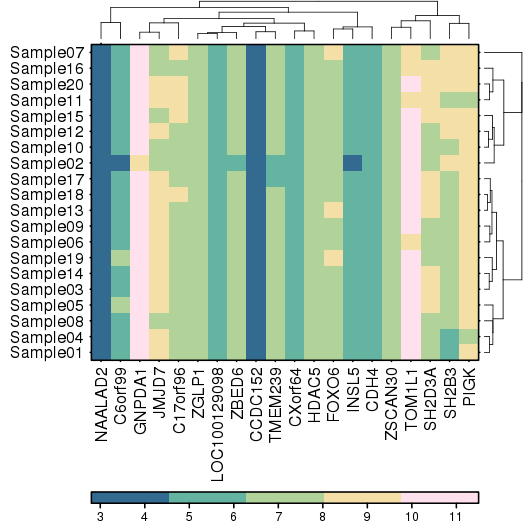
\includegraphics[width=50mm]{Figures/Heatmap_Discrete.png}
     \caption{Heatmap with discrete colours}
  \end{center}
\end{figure}

\subsection{Barplot}
\begin{verbatim}
create.barplot
\end{verbatim}

The barplot is designed to display counts of categorical data. This means data which is divided into discrete bins. 

When displaying data with uncertainty, therefore suggesting the addition of error bars, barplots are not an optimal choice (although, it \textit{is} possible to add error bars to barplots using BL.plotting.general). Barplots are not designed for displaying distributions, and error bars might cover ranges never observed in the data: it is advised that using a boxplot  or a strip plot might be more appropriate \cite{streit}. 

\subsubsection{Simple barplot}
A minimal barplot requires a data frame and corresponding formula.

\begin{verbatim}
# Set up the data
total.counts <- apply(SNV[1:15], 2, function(x){ mutation.count <- (30 - sum(is.na(x)))});
count.nonsyn <- function(x){ mutation.count <- length(which(x == 1)); }
nonsynonymous.SNV <- apply(SNV[1:15], 2, count.nonsyn);
other.mutations <- total.counts - nonsynonymous.SNV;

# Create a data frame 
barplot.data <- data.frame(
    samples = rep(1:15, 2),
    mutation = c(rep("nonsynonymous", 15), rep("other",15)),
    values = c(nonsynonymous.SNV, other.mutations)
    );
    
# Create the simple plot
create.barplot(
    filename = "Barplot_Minimal_Input.png",
    formula = values ~ samples,
    data = barplot.data[barplot.data$mutation == "nonsynonymous",]
    );
\end{verbatim}
\begin{figure}[!ht]
  \begin{center}
     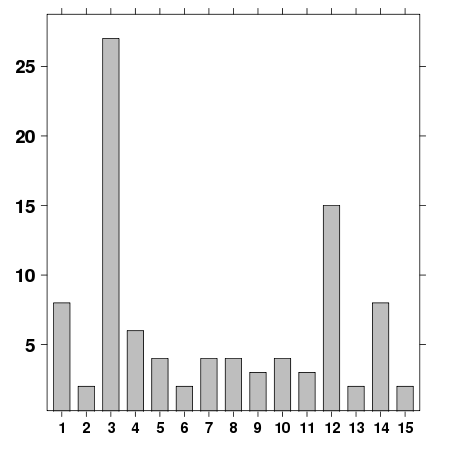
\includegraphics[width=50mm]{Figures/Barplot_Minimal_Input.png}
     \caption{Simple barplot}
  \end{center}
\end{figure}


\subsubsection{Stacked barplot with legend}
Stacked barplots compare overall quantities across items, and also indicate the contribution of sub-categories to the total count \cite{streit}.

\begin{verbatim}
create.barplot(
    filename = "Barplot_Stacked.png",
    formula = values ~ samples,
    data = barplot.data,
    
    # Declaring that the plot will be stacked, not grouped
    stack = TRUE,
    
    # Specify how the data should be divided
    groups = mutation,
    
    # Setting different colours for the groups
    col = default.colours(2, palette.type = "pastel"),
    
    # Creating a legend 
    legend = list(
        inside = list(
            fun = draw.key,
            args = list(
                key = list(
                	
                	  # Here the points in the legends are drawn
                    points = list(
                        col = "black",
                        pch = 22,
                        cex = 2,
                        # reverse order to match stacked bar order
                        fill = rev(default.colours(2, palette.type = "pastel"))
                        ),

                    # Here the text in the legend is drawn
                    text = list(
                        # reverse order to match stacked bar order
                        lab = rev(c("Nonsynonymous SNV", "Other SNV"))
                        ),
                    padding.text = 3,
                    cex = 1
                    )
                ),
            # Where the legend should be placed
            x = 0.55,
            y = 0.95
            )
        )
    );
\end{verbatim}

\begin{figure}[!ht]
  \begin{center}
     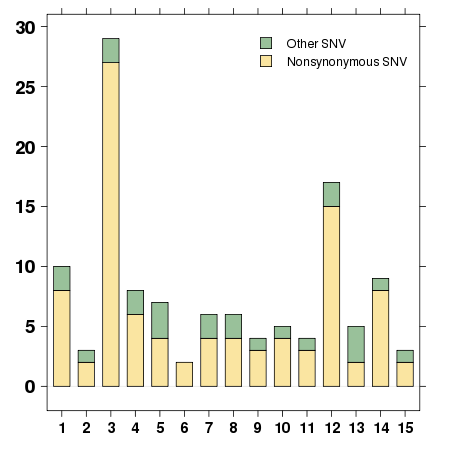
\includegraphics[width=50mm]{Figures/Barplot_Stacked.png}
     \caption{Stacked barplot}
  \end{center}
\end{figure}

\subsubsection{Grouped barplot with legend}
Grouped barplots focus on comparing values across sub-categories, and allow  for comparison across items \cite{streit}.

\begin{verbatim}
create.barplot(
    filename = "Barplot_Grouped.png",
    formula = values ~ samples,
    data = barplot.data,
    
    # Specifying how the data will be divided
    # Defaults to creating grouped bar plots when this is set
    groups = mutation,
    
    # Setting colours for the groups
    col = default.colours(2, palette.type = "pastel"),
    
    # Creating a legend 
    legend = list(
        inside = list(
            fun = draw.key,
            args = list(
                key = list(
                	
                	  # Here the points in the legends are drawn
                    points = list(
                        col = "black",
                        pch = 22,
                        cex = 2,
                        fill = default.colours(2, palette.type = "pastel")
                        ),

                    # Here the text in the legend is drawn
                    text = list(
                        lab = c("Nonsynonymous SNV", "Other SNV")
                        ),

                    # Spacing between items
                    padding.text = 3,
                    cex = 1
                    )
                ),
            # Where on the plotting space the legend should be placed
            x = 0.55,
            y = 0.95
            )
        )
    );
\end{verbatim}

\begin{figure}[!ht]
  \begin{center}
     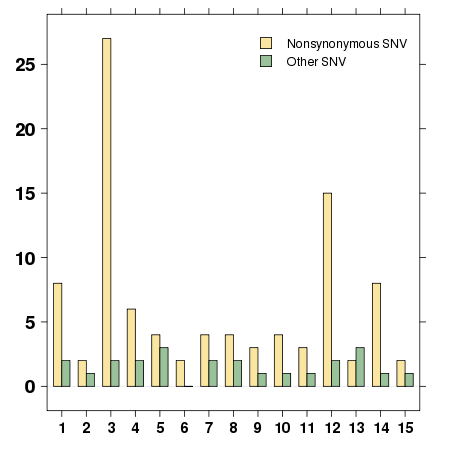
\includegraphics[width=50mm]{Figures/Barplot_Grouped.png}
     \caption{Grouped barplot}
  \end{center}
\end{figure}

\subsection{Density plot}
\begin{verbatim}
create.densityplot
\end{verbatim}

The density plot also shows data distributions. It is an empirical estimate of the probability density function, and the area under the curve is the cumulative distribution function. It can be thought of as a smoothed version of the histogram.

In comparison to the boxplot, the density plot can compare fewer distributions because after a certain point the lines will interfere with one another. Additionally, summary statistics are not directly provided by the density plot. However, the density plot reveals more subtleties in the ``shape" of the data, which may be hidden in the boxplot.

\subsubsection{Simple density plot}
The minimal input required by a density plot is a list of vectors.

\begin{verbatim}
create.densityplot(
    filename = "Densityplot_Minimal_Input.png",
    x = as.data.frame(t(microarray[1:3,1:58]))
    );
\end{verbatim}

\begin{figure}[!ht]
  \begin{center}
     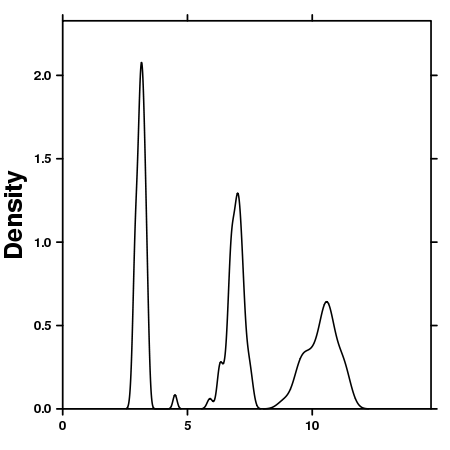
\includegraphics[width=50mm]{Figures/Densityplot_Minimal_Input.png}
     \caption{Simple density plot}
  \end{center}
\end{figure}

\subsubsection{Density plot with line type}
Different colours and line types can be used to better distinguish between the lines

\begin{verbatim}
create.densityplot(
    filename = "Densityplot_Lty.png",
    x = as.data.frame(t(microarray[1:3,1:58])),
    
    # Line type
    lty = c("solid", "dashed", "dotted"),
    
    # Colours
    col = default.colours(3)
    );
\end{verbatim}

\begin{figure}[!ht]
  \begin{center}
     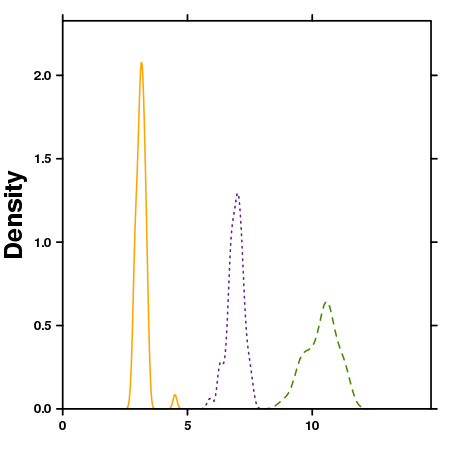
\includegraphics[width=50mm]{Figures/Densityplot_Lty.png}
     \caption{Density plot with colour and line type}
  \end{center}
\end{figure}

\subsection{Dendrogram}
\begin{verbatim}
create.dendrogram
\end{verbatim}

The dendrogram is a tree diagram used to display the clustering arrangement determined by hierarchical clustering. It is often used in conjunction with heatmaps to indicate the clustering of genes or samples. In BL.plotting.general, this function is called by the \verb|create.heatmap| function when cells are clustered.

The distance from a leaf node to a node indicates the correlation to other leaf nodes, where further distances indicate less correlation. Closely clustered leaf nodes (located at the bottom of the dendrogram) are highly correlated.

\subsubsection{Simple dendrogram}
This function is not structured the same way as other plotting functions. It does not create Trellis objects, and is not usually plotted alone.

\begin{verbatim}
dendrogram <- create.dendrogram(x = microarray[1:20, 1:20]);
png("Dendrogram_Simple.png");
plot(x = dendrogram);
dev.off();

\end{verbatim}
\begin{figure}[!ht]
  \begin{center}
     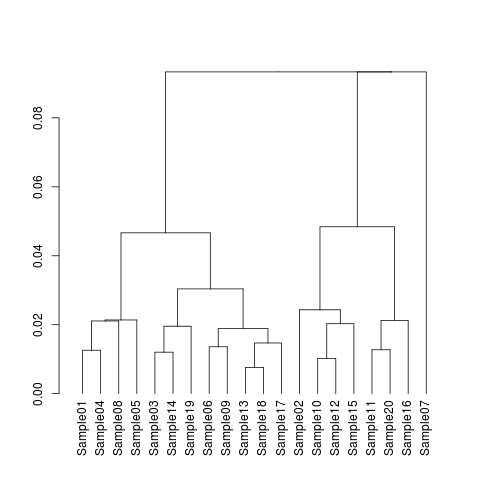
\includegraphics[width=50mm]{Figures/Dendrogram_Simple.png}
     \caption{Simple dendrogram}
  \end{center}
\end{figure}

\subsection{Dotmap}
\begin{verbatim}
create.dotmap
\end{verbatim}

The dotmap is a novel chart-type found in BL.plotting.general. It is a matrix of dots, where the dot sizes and dot colours are used to encode information. The matrix can also be filled with a background colour, similar to heatmaps. This plot is very useful for displaying high-dimensional data because it is able to display two dimensions more than a heatmap through dot size and dot colour.

One example of how to use this plot is to use the dot size to indicate magnitude of fold change, dot colour to show the direction of change, and the background colour to indicate p-values.

\subsubsection{Simple dotmap}
A basic dotmap takes a data frame as input.
\begin{verbatim}
# Generating fake data
dotmap.data <- data.frame(
    "A" = runif(n = 10, min = -1, max = 1),
    "B" = runif(n = 10, min = -1, max = 1),
    "C" = runif(n = 10, min = -1, max = 1)
    );

# Functions to decide the spot size and colour can be included
# If not, default functions will be used
spot.size.function <- function(x) { 0.1 + (2 * abs(x)); }

spot.colour.function <- function(x) {
    colours <- rep("white", length(x));
    colours[sign(x) == -1] <- default.colours(2, palette.type = "dotmap")[1];
    colours[sign(x) ==  1] <- default.colours(2, palette.type = "dotmap")[2];
    return(colours);
    }

create.dotmap(
    filename = "Dotmap_Simple.png",
    x = dotmap.data
    );
\end{verbatim}

\begin{figure}[!ht]
  \begin{center}
     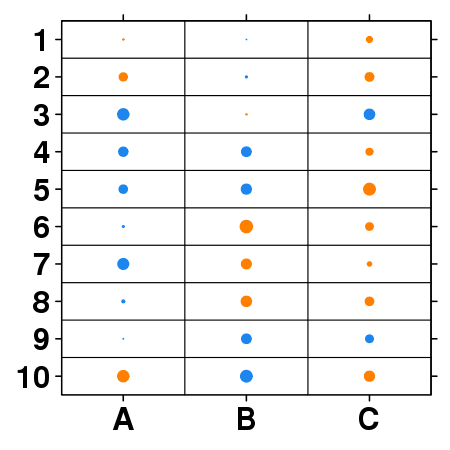
\includegraphics[width=50mm]{Figures/Dotmap_Simple.png}
     \caption{Simple dotmap}
  \end{center}
\end{figure}

\subsubsection{Dotmap with legend}
A legend can be added to indicate the meaning of the dot colours and sizes.

\begin{verbatim}
create.dotmap(
    filename = "Dotmap_Legend.png",
    x = dotmap.data,
    
    # Using the specified spot size and colour functions
    spot.size.function = spot.size.function,
    spot.colour.function = spot.colour.function,    
    
    # Create a legend matching the dot sizes
    key = list(
    
        # This indicates which side of the plot the legend will appear
        space = "right",
        
        # Here the points are created using the spot size and colour functions
        # This ensures that they match the spots found in the plot
        points = list(
            cex = spot.size.function(seq(-1, 1, 0.2)),
            col = spot.colour.function(seq(-1, 1, 0.2)),
            pch = 19
            ),
        
        # These are the labels which will match the dots
        text = list(
            lab = c("-1.0", "-0.8", "-0.6", "-0.4", "-0.2", " 0.0", "+0.2",
                 "+0.4", "+0.6", "+0.8", "+1.0"),
            cex = 1.5,
            adj = 1.0,
            fontface = "bold"
            )
        )
    );
\end{verbatim}

\begin{figure}[!ht]
  \begin{center}
     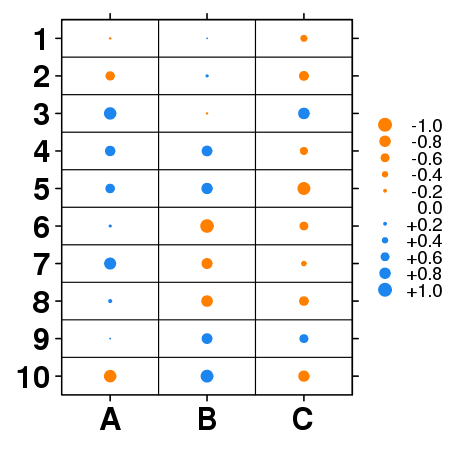
\includegraphics[width=50mm]{Figures/Dotmap_Legend.png}
     \caption{Dotmap with legend}
  \end{center}
\end{figure}

\subsubsection{Dotmap with background}
The background of each cell can also have a colour. Colours do not appear the same with and without borders \cite{brewer-colour}. Therefore it is advisable to keep the surrounding colours of points consistent between the legend and the plotting space.

\begin{verbatim}
# Generating background data
bg.data <- data.frame(
    "A" = runif(n = 10, min = -1, max = 1),
    "B" = runif(n = 10, min = -1, max = 1),
    "C" = runif(n = 10, min = -1, max = 1)
    );

create.dotmap(
    filename = "Dotmap_Background.png",
    x = dotmap.data,
    spot.size.function = spot.size.function,
    spot.colour.function = spot.colour.function,    
    key = list(
        space = "right",
        points = list(
            cex = spot.size.function(seq(-1, 1, 0.2)),
            col = spot.colour.function(seq(-1, 1, 0.2)),
            pch = 19
            ),
        text = list(
            lab = c("-1.0", "-0.8", "-0.6", "-0.4", "-0.2", " 0.0", "+0.2", 
                "+0.4", "+0.6", "+0.8", "+1.0"),
            cex = 1.5,
            adj = 1.0,
            fontface = "bold"
            )
        ),
    
    # Control spacing at top of key
    key.top = 1,

    # Adding border to points to stand out more from background
    pch = 21,
    pch.border.col = "white",
    
    # Adding the background
    bg.data = bg.data,

    # Adding a colourkey
    colourkey = TRUE,
    
    # Setting colour scheme for background data
    colour.scheme = c("white", "black"),
    
    # Making bg colour scheme a discrete colour scheme, with breaks at these places
    at = seq(-1, 1, 0.5)
    );
\end{verbatim}

\begin{figure}[!ht]
  \begin{center}
     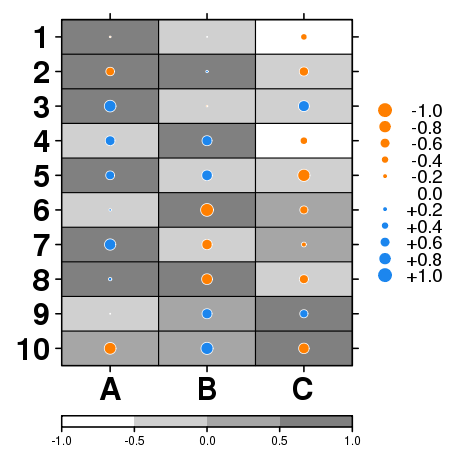
\includegraphics[width=50mm]{Figures/Dotmap_Background.png}
     \caption{Dotmap with background}
  \end{center}
\end{figure}

\subsection{Hexbinplot}
\begin{verbatim}
create.hexbinplot
\end{verbatim}

The hexbinplot is a hexagonally binned plot which uses colour (usually colour value) to plot points. It uses a coordinate grid similar to scatterplots, but while scatterplots display individual data points, the hexbinplot displays the density of data points in a given space on the plot. It might be thought of as similar to a two-dimensional histogram. One use-case for this plot is in circumstances where data points are too densely packed to be distinguishable on a scatterplot.

\subsubsection{Simple hexbinplot}
The minimum input for a hexbinplot is data frame and formula.
\begin{verbatim}
hexbin.data <- data.frame(
    x = microarray[,1],
    y = microarray[,2]
    );
    
create.hexbinplot(
    filename = "Hexbin_Simple.png",
    data = hexbin.data,
    formula = x ~ y
    );
\end{verbatim}

\begin{figure}[!ht]
  \begin{center}
     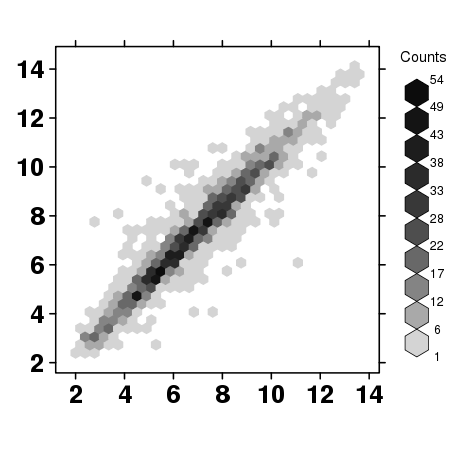
\includegraphics[width=50mm]{Figures/Hexbin_Simple.png}
     \caption{Simple hexbinplot}
  \end{center}
\end{figure}

\subsubsection{Hexbinplot with custom bins}
The bin sizes can be customized to use more standard increments.
\begin{verbatim}
create.hexbinplot(
    filename = "Hexbin_Bins.png",
    data = hexbin.data,
    formula = x ~ y, 

    # Setting the number of bins
    xbins = 15,
    colourcut = seq(0, 1, length = 9),
    maxcnt = 160
    );
\end{verbatim}

\begin{figure}[!ht]
  \begin{center}
     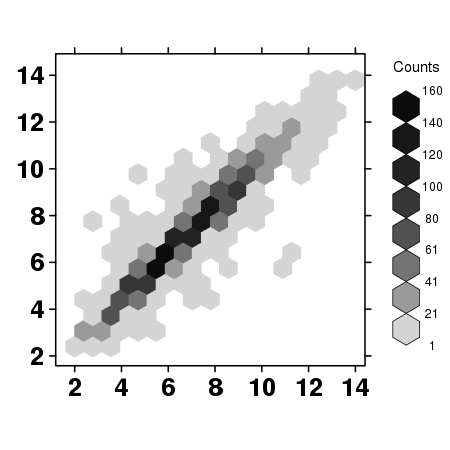
\includegraphics[width=50mm]{Figures/Hexbin_Bins.png}
     \caption{Hexbinplot with custom bins}
  \end{center}
\end{figure}

\subsection{Histogram}
\begin{verbatim}
create.histogram
\end{verbatim}

The histogram represents the distribution of data. It is an estimation of the probability distribution of a continuous variable. If a histogram had an infinite number of bars, it would have the same shape as a density plot. 

Although its appearance is similar to a barplot, the main difference is that a barplot uses discrete data, while a histogram uses continuous data. This means that the `bins' of a histogram are data-ranges. This points to why the bars in a barplot are often separated by a space, while the bars in a histogram are usually directly next to one another.

\subsubsection{Simple histogram}
The minimal input for the histogram is either a numeric vector, or a formula and data frame.
\begin{verbatim}
create.histogram(
    filename = "Histogram_Minimal_Input.png",
    x = microarray[,1]
    );
\end{verbatim}

\begin{figure}[!ht]
  \begin{center}
     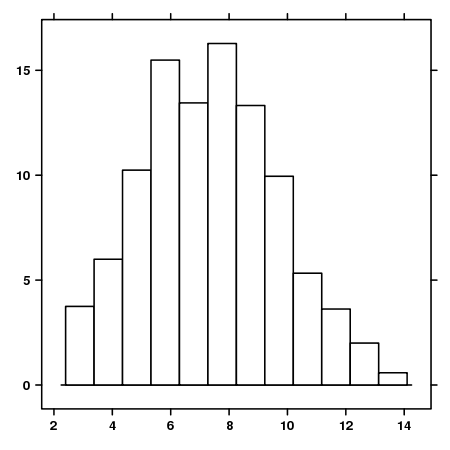
\includegraphics[width=50mm]{Figures/Histogram_Minimal_Input.png}
     \caption{Simple histogram}
  \end{center}
\end{figure}

\subsection{Manhattan plot}
\begin{verbatim}
create.manhattanplot
\end{verbatim}

The Manhattan plot is a type of scatterplot used to display chromosomal locations along the x-axis, and the negative logarithm of p-values of mutations along the y-axis. This means that the points which are higher on the plot are highly significant, while the points near the 0 axis are less significant.

\subsubsection{Simple Manhattan plot}
This plot accepts a data frame together with a formula for the x and y components. Manhattan plots usually display a large number of data points.

\begin{verbatim}
# Generating some fake example data
manhattan.data <- data.frame(
    x = runif(20000, 0, 1),
    y = 1:20000
    );

create.manhattanplot(
    filename = "Manhattan_Simple.png",
    formula = -log10(x) ~ y,
    data = manhattan.data
    );
\end{verbatim}

\begin{figure}[!ht]
  \begin{center}
     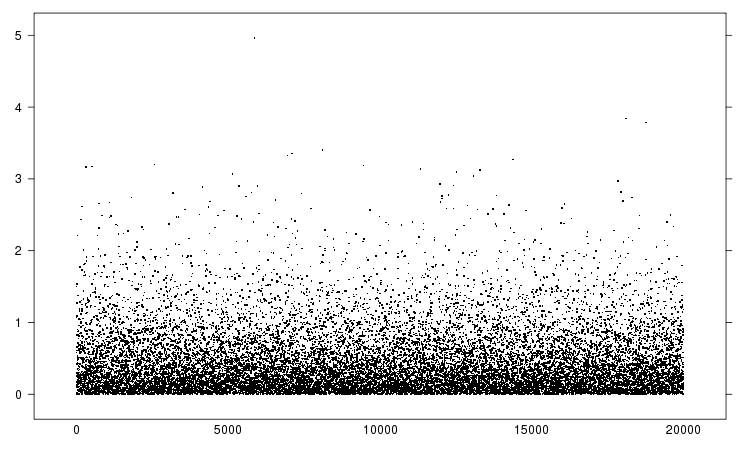
\includegraphics[width=50mm]{Figures/Manhattan_Simple.png}
     \caption{Simple Manhattan plot}
  \end{center}
\end{figure}

\subsubsection{Manhattan plot with line}
Adding a line can be used to easily view data points above a particular p-value.

\begin{verbatim}
create.manhattanplot(
    filename = "Manhattan_Line.png",
    formula = -log10(x) ~ y,
    data = manhattan.data,
    
    # Adding a horizontal line
    abline.h = 2,
    
    # Changing the line type and style
    abline.col = "red",
    abline.lwd = 3,
    abline.lty = "solid"
    );
\end{verbatim}

\begin{figure}[!ht]
  \begin{center}
     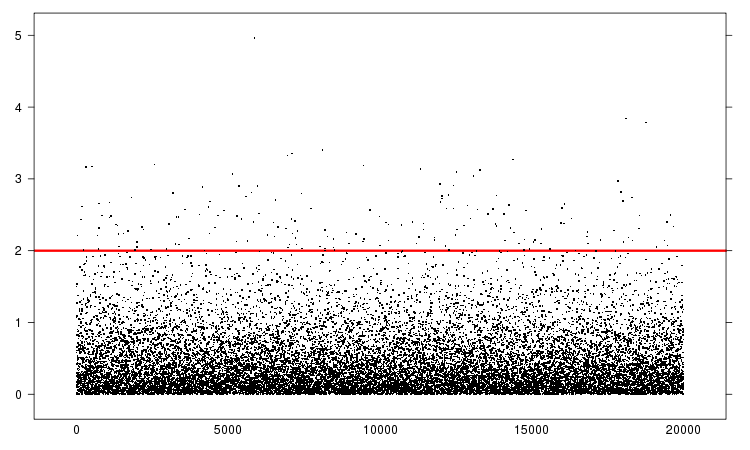
\includegraphics[width=50mm]{Figures/Manhattan_Line.png}
     \caption{Manhattan plot with line}
  \end{center}
\end{figure}


\subsection{Polygon plot}
\begin{verbatim}
create.polygonplot
\end{verbatim}

The polygon plot draws a polygon. There are many options for how to use this function. It takes as input the maximum and minimum values and optional median values, and fills in the difference to be the polygon `shape'. This chart is often used for repeated, iterative data, such as time-series data.

\subsubsection{Simple polygon plot}
The minimum input for a polygon plot is data frame and formula to extract the components. Additional input is needed to determine the maximum and minimum values of the polygon, as well as the optional median values.

\begin{verbatim}
# Generating fake data
set.seed(12345);
temp  <- matrix(runif(1010), ncol = 10) + sort(runif(101));

polygon.data <- data.frame(
    x = 0:100,
    max = apply(temp, 1, max),
    min = apply(temp, 1, min)
    );

# Creating the simple plot
create.polygonplot(
    filename = "Polygon_Simple.png",
    formula = NA ~ x,
    data = polygon.data,
    max = polygon.data$max,
    min = polygon.data$min,

    # Adjusting the axes limits
    xlimits = c(0,100),
    ylimits = c (0,2),
    
    # Adding fill colour
    col = default.colours(1, palette.type = "pastel")
    );
\end{verbatim}

\begin{figure}[!ht]
  \begin{center}
     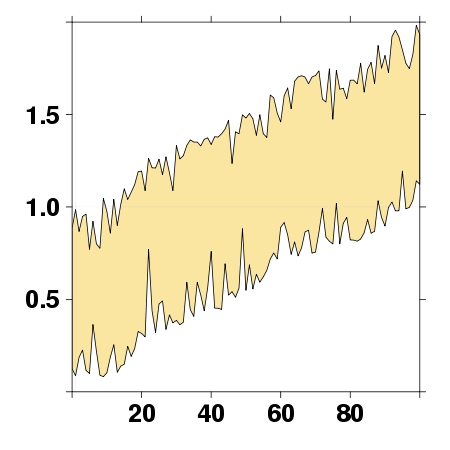
\includegraphics[width=50mm]{Figures/Polygon_Simple.png}
     \caption{Simple polygon plot}
  \end{center}
\end{figure}

\subsection{Quantile-quantile plot}
A quantile-quantile plot compares distributions by plotting them in a scatterplot fashion, where one distribution provides the x-axis values, and the other distribution provides the y-axis values. The closer in appearance the plot is to an y = x line indicates how similar the two distributions are.

\begin{verbatim}
create.qqplot.comparison
\end{verbatim}
This quantile-quantile plot compares two distributions.
\begin{verbatim}
create.qqplot.fit
\end{verbatim}
This quantile-quantile plot compares a distribution against a theoretical distribution.

\subsubsection{Simple QQ plot comparison}
The minimum input for the QQ plot comparison is either a list of numeric vectors or a data source and formula.
\begin{verbatim}
create.qqplot.comparison(
    filename = "QQcomparison_Simple.png",
    x = list(rnorm(100), rnorm(100))
    );
\end{verbatim}

\begin{figure}[!ht]
  \begin{center}
     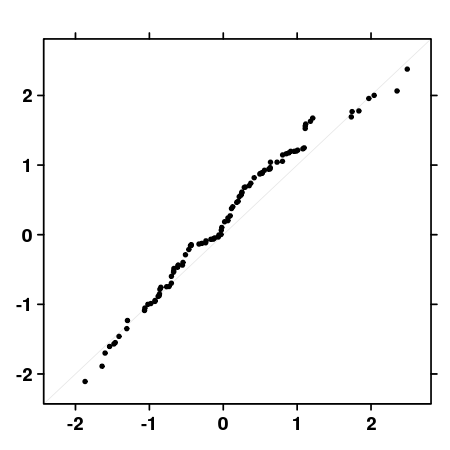
\includegraphics[width=50mm]{Figures/QQcomparison_Simple.png}
     \caption{Simple qqplot comparison}
  \end{center}
\end{figure}

\subsubsection{Simple QQ plot fit}
The minimum input for the QQ plot fit is either a list of numeric vectors or a data source and formula.

\begin{verbatim}
create.qqplot.fit(
    filename = "QQfit_Simple.png",
    x = rnorm(300),
    
    # choosing to compare against a uniform distribution
    distribution = qunif
    );
\end{verbatim}

\begin{figure}[!ht]
  \begin{center}
      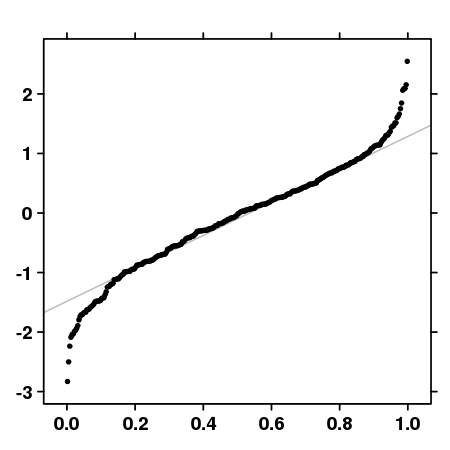
\includegraphics[width=50mm]{Figures/QQfit_Simple.png}
      \caption{Simple qqplot fit}
  \end{center}
\end{figure}

\subsection{Segplot}
\begin{verbatim}
create.segplot
\end{verbatim}

The segplot is also known as a forest plot, and is often used to compare the effectiveness of treatments suggested by different studies, but can be applied to a variety of other datasets. The middle value can be used to indicate a point, while the bar may show the surrounding range of values. This kind of plot can be used to compare distributions, where summary statistics are displayed.

\subsubsection{Simple segplot}
The minimum input to a segplot is a data frame and corresponding formula.

\begin{verbatim}
# Generating fake data
segplot.data <- data.frame(
    min = runif(10,5,15),
    max = runif(10,15,25),
    labels = as.factor(LETTERS[1:10])
    );

create.segplot(
    filename = "Segplot_simple.png",
    formula = labels ~ min + max,
    data = segplot.data
    );
\end{verbatim}

\begin{figure}[!ht]
  \begin{center}
     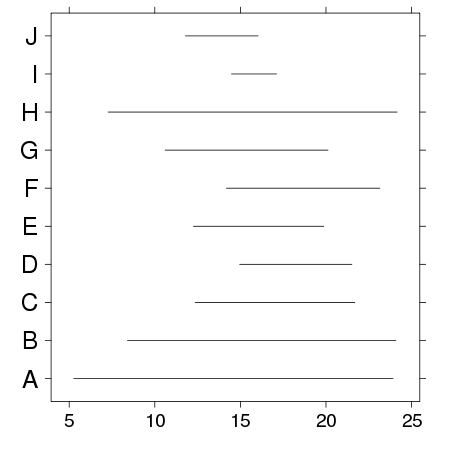
\includegraphics[width=50mm]{Figures/Segplot_simple.png}
     \caption{Simple segplot}
  \end{center}
\end{figure}

\subsubsection{Segplot with bands}
Segplots can be displayed using thick bands.

\begin{verbatim}
create.segplot(
    filename = "Segplot_bands.png",
    formula = labels ~ min + max,
    data = segplot.data,
    
    # Using bands instead of lines
    draw.bands = TRUE
    );
\end{verbatim}

\begin{figure}[!ht]
  \begin{center}
     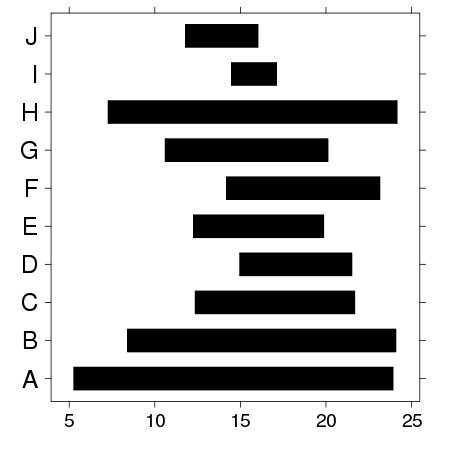
\includegraphics[width=50mm]{Figures/Segplot_bands.png}
     \caption{Segplot with bands}
  \end{center}
\end{figure}

\subsection{Strip plot}
\begin{verbatim}
create.stripplot
\end{verbatim}

The strip plot is a type of scatterplot where one axis is discrete, meaning that the points are divided into discrete bins. If points are densely packed, they can be more easily distinguished by applying a jitter. This kind of plot can be used to display distributions, where each data point is shown.

\subsubsection{Simple strip plot}
The minimum input for a strip plot is a data frame and formula indicating x and y components.
\begin{verbatim}
stripplot.data <- data.frame(
    values = c(t(microarray[1:10, 1:58])),
    genes = rep(rownames(microarray)[1:10], each = 58)
    );

create.stripplot(
    filename = "Stripplot_Minimal_Input.png",
    formula = genes ~ values,
    data = stripplot.data
    );
\end{verbatim}

\begin{figure}[!ht]
  \begin{center}
	 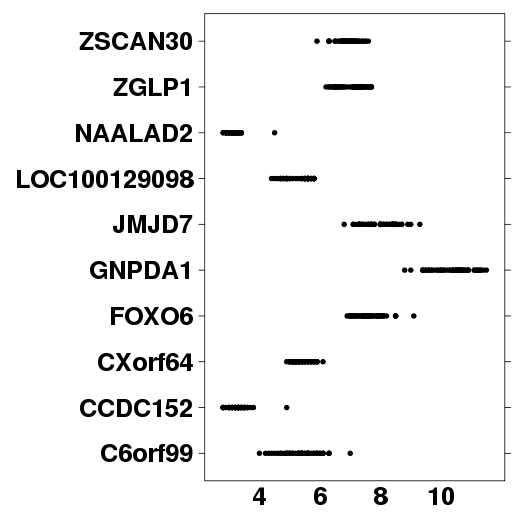
\includegraphics[width=50mm]{Figures/Stripplot_Minimal_Input.png} 
    \caption{Simple stripplot}
  \end{center}
\end{figure}

\subsubsection{Strip plot with jitter}
Adding jitter to the points can make it easier to distinguish the values in a strip plot.
\begin{verbatim}
create.stripplot(
    filename = "Stripplot_Jitter.png",
    formula = genes ~ values,
    data = stripplot.data,
    
    # Adding jitter
    # The amount of jitter used can be controlled using jitter.factor and jitter.amount
    jitter.data = TRUE
    );
\end{verbatim}

\begin{figure}[!ht]
  \begin{center}
	 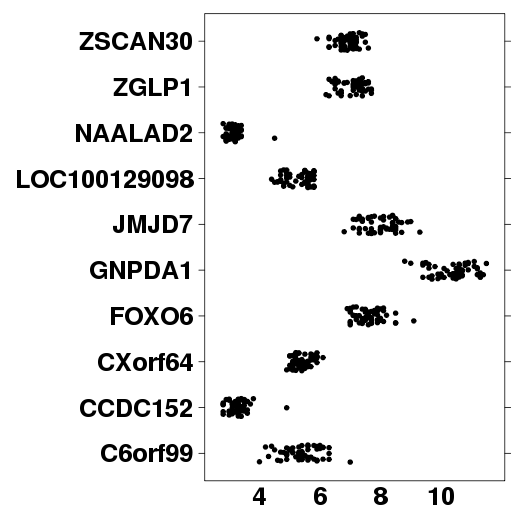
\includegraphics[width=50mm]{Figures/Stripplot_Jitter.png} 
    \caption{Stripplot with jitter}
  \end{center}
\end{figure}

\subsection{Violin plot}
\begin{verbatim}
create.violinplot
\end{verbatim}

The violin plot is a combination of a boxplot and a kernel density plot. The shape of the violin plot shows the density, where wider sections of the plot indicate regions of higher density. Additional optional points within the violins can be used to encode the median and interquartile range. This is a method of comparing distributions where both summary statistics and a visualization of the data is provided. One difference with this method compared to the density plot is that the violin plot does not indicate what the actual density values are: the height or width of bulges in the violin plots is relative, not absolute.

\subsubsection{Simple violin plot}
The minimal input for a violin plot is a data frame and formula.
\begin{verbatim}
violin.data <- data.frame(
    values = c(t(microarray[1:10, 1:58])),
    genes = rep(rownames(microarray)[1:10], each = 58)
    );

create.violinplot(
    filename = "Violinplot_Minimal_Input.png",
    formula = values ~ genes,
    data = violin.data,

    # Rotating the axes labels to be clearer
    xaxis.rot = 90
    );
\end{verbatim}

\begin{figure}[!ht]
  \begin{center}
     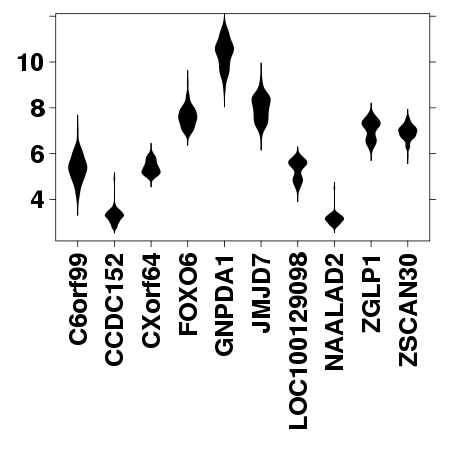
\includegraphics[width=50mm]{Figures/Violinplot_Minimal_Input.png}
     \caption{Simple violinplot}
  \end{center}
\end{figure}

\section{Multiplot}
\begin{verbatim}
create.multiplot
\end{verbatim}

The muliplot is not a chart-type in itself: rather, it is a function to combine multiple plots into a single plot. It enables the creation of complex figures in a programmable way and encourages good design by standardizing elements such as line widths and font size. 

\subsection{Example 1: Simple multiplot}
This example creates a figure out of a single bar plot and three heatmaps using the HairEyeColor data set supplied by the R datasets package.

\begin{figure}[!ht]
  \begin{center}
     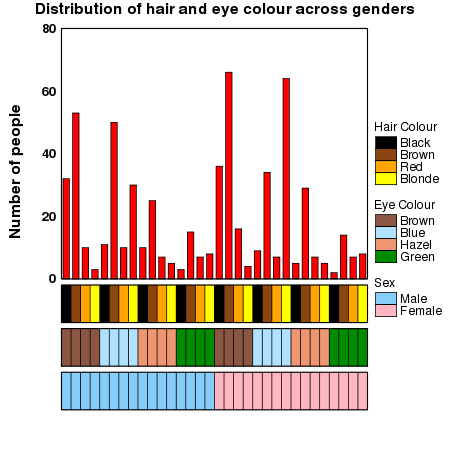
\includegraphics[width=70mm]{Figures/Multiplot_Ex1.png}
     \caption{Example 1 multiplot}
     \label{fig:picture}
  \end{center}
\end{figure}

\subsubsection{Setting up the data}
The first step is to format the data. 

\begin{verbatim}
# Put the array into a data frame that will be used in the barplot
haireye <- as.data.frame(HairEyeColor);

# put each column of the dataframe into a matrix for the heatmap
Hair <- as.matrix(as.numeric(haireye[,1]));
Eye <- as.matrix(as.numeric(haireye[,2]));
Sex <- as.matrix(as.numeric(haireye[,3]));
\end{verbatim}

\subsubsection{Creating the bar plot}
The code below creates a bar plot showing the number of males and females with a particular hair and eye colour. Proper labels and titles will be added at the end using the create.multiplot function. The plot is not printed to file -- instead, it is saved in the \verb|hair.eye.colour.barplot| variable for later use by the multiplot function.

\begin{verbatim}
# create the barplot used for the frequency of each type of person
hair.eye.colour.barplot <- create.barplot(
        formula = Freq ~ c(1:32),
        data = haireye,
        col = "red",

        # Set the limits that the plot will display to 0 and 80 to make it look nicer
        ylimits = c(0.00, 80)
        );
\end{verbatim}

\begin{figure}[!ht]
  \begin{center}
     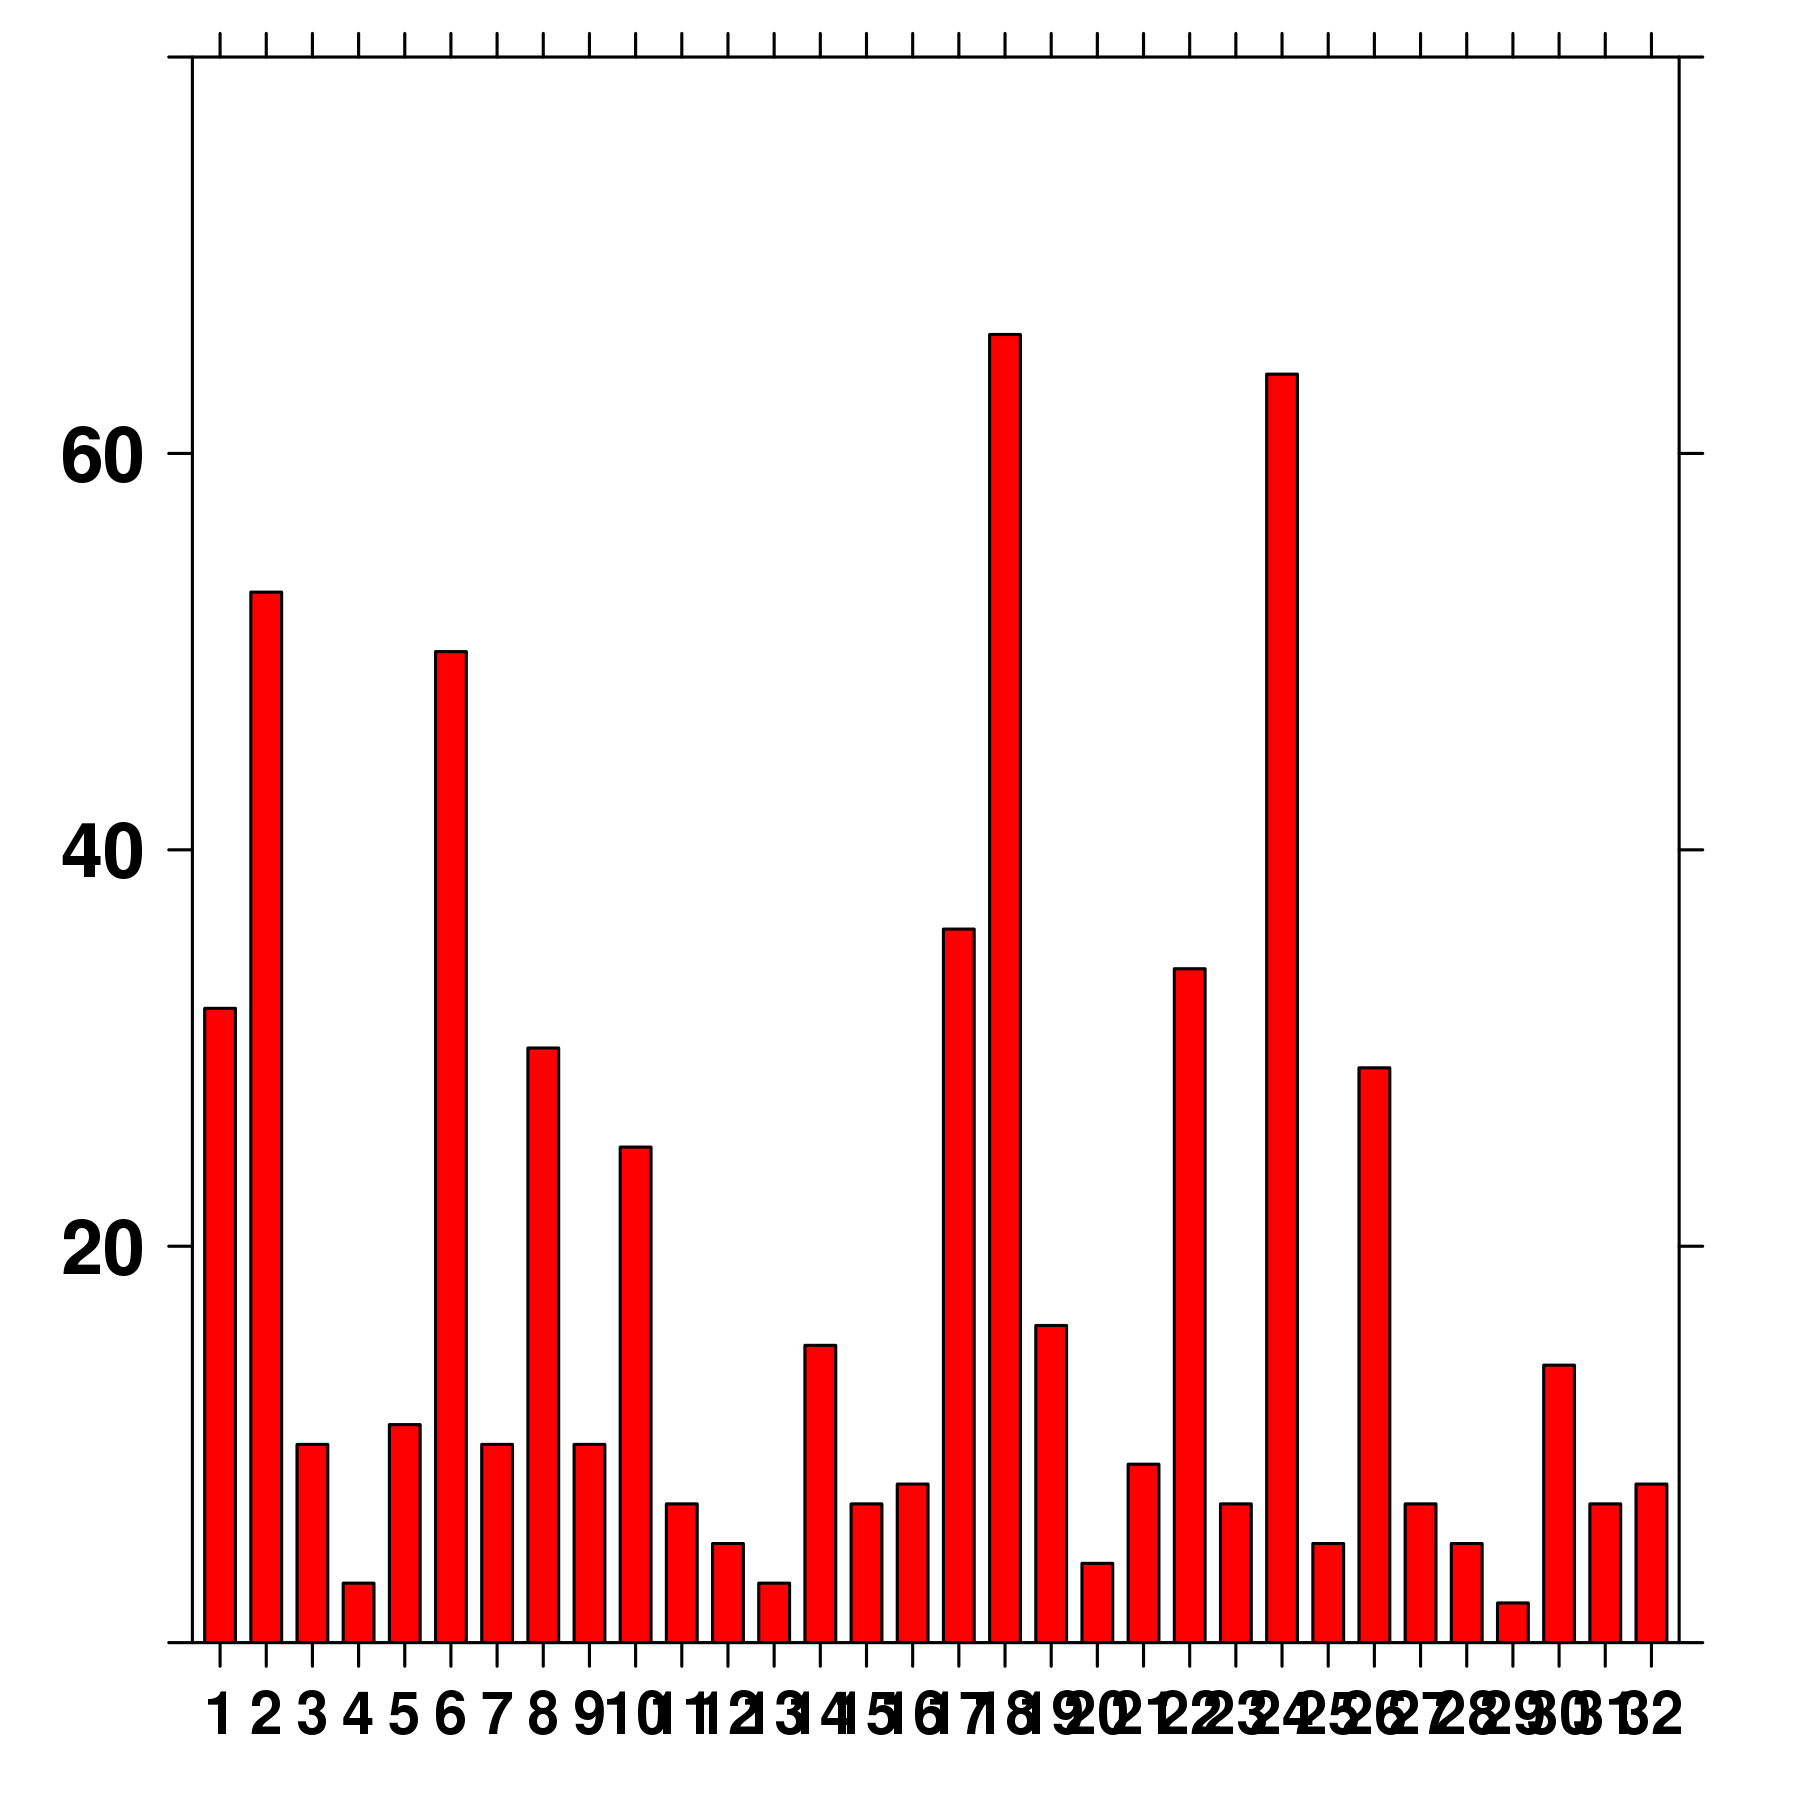
\includegraphics[width=50mm]{Figures/ex1_barplot.png}
     \caption{Hair and eye colour barplot}
     \label{fig:picture}
  \end{center}
\end{figure}

\subsubsection{Creating the covariate bars}
The covariate bars in this example are created using the create.heatmap function.  Discrete colour schemes are used in these covariate bars, and each colour used in specified in the colour.scheme parameter. The total number of colours used is specified in the total.col parameter, plus one to account for the white which is displayed in the case of missing values.

\begin{verbatim}
hair.heatmap <- create.heatmap(
        x = Hair,
        clustering.method = "none",
        scale.data = FALSE,
        colour.scheme = c("black", "chocolate4", "orange", "yellow"),
    
        # Show each of those colours once (i.e, four values, four colours)
        total.col = 5,
        grid.col = TRUE,
        print.colour.key = FALSE,

        # Remove y-axis ticks
        yaxis.tck = 0,
        height = 1
        );
\end{verbatim}

\begin{figure}[!ht]
  \begin{center}
     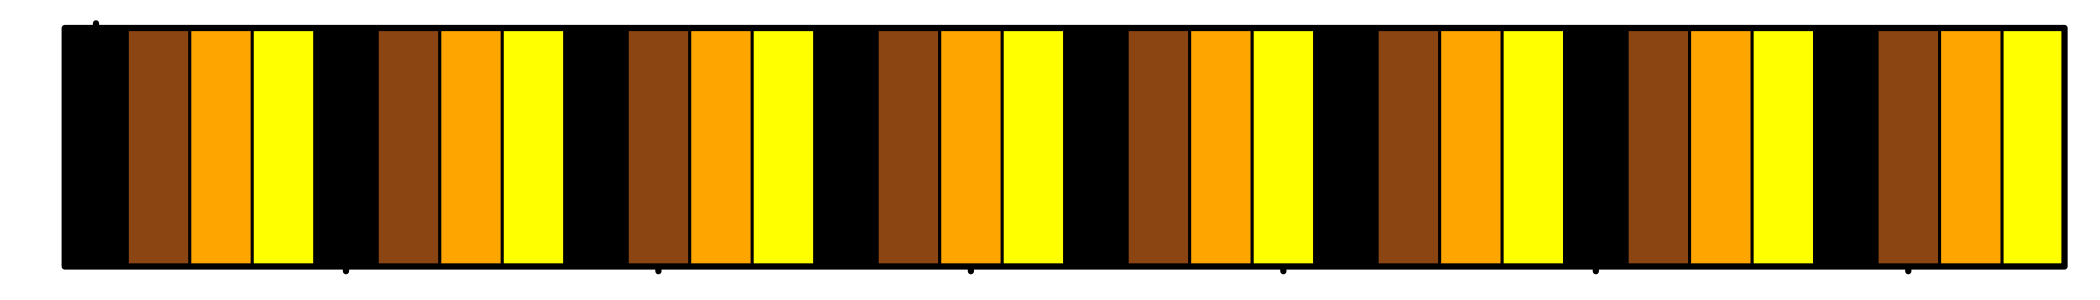
\includegraphics[width=50mm]{Figures/ex1_hair_heatmap.png}
     \caption{Hair colour covariate}
     \label{fig:picture}
  \end{center}
\end{figure}

The same process is followed for the remaining covariate bars.

\begin{verbatim}
eye.heatmap <- create.heatmap(
        x = Eye,
        clustering.method = "none",
        scale.data = FALSE, 
        colour.scheme = c("lightsalmon4", "lightskyblue1", "lightsalmon2", "green4"),
        total.col = 5,
        grid.col = TRUE,
        print.colour.key = FALSE,
        yaxis.tck = 0,
        height = 1
        );
\end{verbatim}

\begin{figure}[!ht]
  \begin{center}
     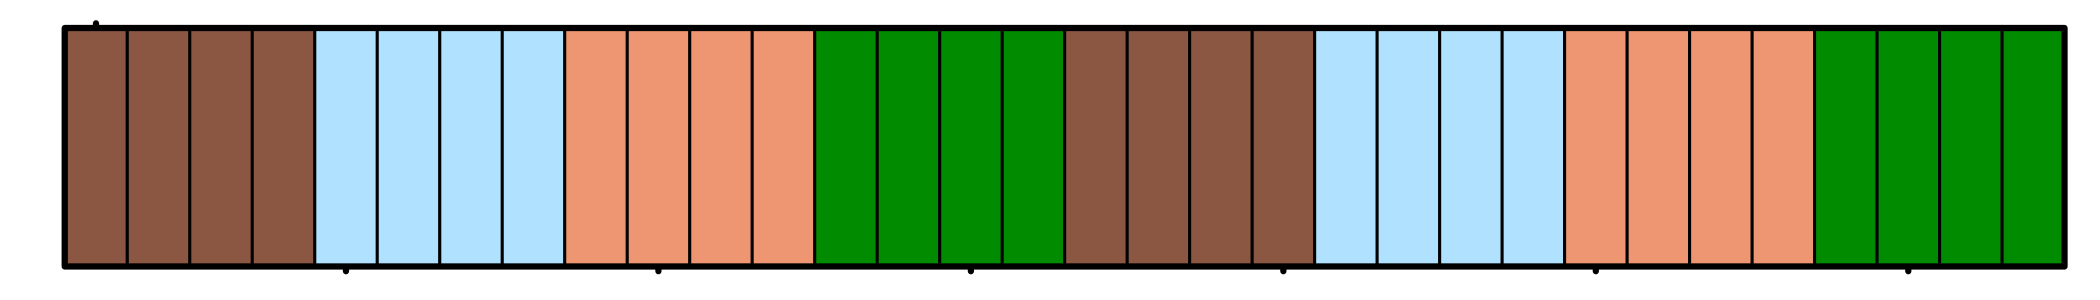
\includegraphics[width=50mm]{Figures/ex1_eye_heatmap.png}
     \caption{Eye colour covariate}
     \label{fig:picture}
  \end{center}
\end{figure}

\begin{verbatim}
sex.heatmap <- create.heatmap(
        x = Sex,
        clustering.method = "none",
        scale.data = FALSE,
        colour.scheme = force.colour.scheme(c("Male","Female"),scheme = "sex"),
        total.col = 3,
        grid.col = TRUE,
        print.colour.key = FALSE,
        yaxis.tck = 0,
        height = 1
        );
\end{verbatim}

\begin{figure}[!ht]
  \begin{center}
     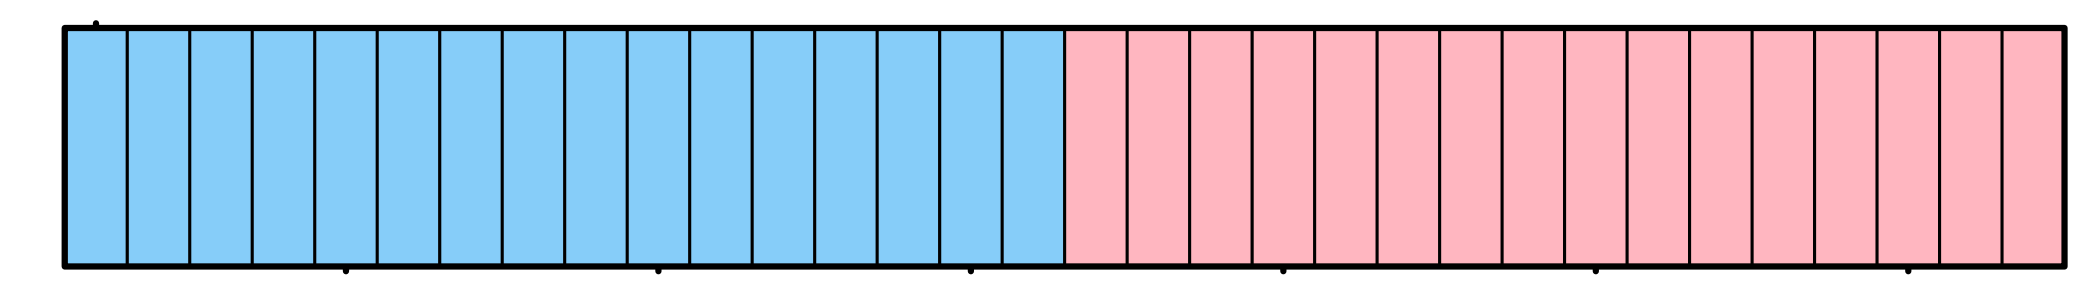
\includegraphics[width=50mm]{Figures/ex1_sex_heatmap.png}
     \caption{Sex covariate}
     \label{fig:picture}
  \end{center}
\end{figure}

\subsubsection {Creating the legend}
A legend is created to differentiate the meaning of the heatmaps. This legend has three sections: one for hair colour, eye colour and sex.

\begin{verbatim}
# create the legend that will be used to show the values of the covariates
legends <- legend.grob( list(

       # create the legend for the hair colour
       legend = list(
               colours = c("black", "chocolate4", "orange", "yellow"),
               title = "Hair Colour",
               labels = c("Black", "Brown", "Red", "Blonde"),
               size = 3,
               title.cex = 2,
               label.cex = 2
               ),

       # create the legend for the eye colour
       legend = list(
               colours = c("lightsalmon4", "lightskyblue1", "lightsalmon2", "green4"),
               title = "Eye Colour",
               labels = c("Brown", "Blue", "Hazel", "Green"),
               size = 3,
               title.cex = 2,
               label.cex = 2
               ),

       # create the legend for the sex
       legend = list(
               colours = force.colour.scheme(c("Male", "Female"),scheme = "sex"),
               title = "Sex",
               labels = c("Male", "Female"),
               size = 3,
               title.cex = 2,
               label.cex = 2
               )
       ), 
       title.just = "left", 
       title.fontface = "plain")
\end{verbatim}

\subsubsection{Creating the final figure}
After all the plots and legends are created, they are combined using the create.multiplot function. This figure is arranged so the bar plot is the largest and at the top, and the three heatmaps appear underneath to explain what each of the covariate bars represent. The order is achieved through listing the plots in the order in which they should appear (from bottom to top) in the plot.objects parameter. Furthermore, axis labels are only on the barplot, leaving others without labels and tick marks.

\begin{verbatim}
 create.multiplot(
    
         # The four plots are listed from bottom to top 
         plot.objects = list(sex.heatmap, eye.heatmap, hair.heatmap, hair.eye.colour.barplot),
         filename = "Multiplot_Ex1.png",
         main = "Distribution of hair and eye colour across genders",

         # The labels are placed on the side of the multiplot 
         # (tabs are needed for labels to be in proper location)
         ylab.label = c("\t", "Number of people", "\t", "\t"),
         main.key.padding = 2,
         ylab.cex = 1.25,
         main.cex = 1.25,
         yaxis.cex = 1,
         panel.heights = c(1, 0.15, 0.15, 0.15),

         # The spacing between the plots is set so there is very little space between heat graphs
         yspacing = c(-1, -1, -1),
         xaxis.lab = NULL,

         # Remove axes tick marks
         xaxis.alternating = 0,
         yaxis.alternating = 0,

         # Set the yaxis labels (only needed on the bar plot)
         yaxis.lab = list(NULL, NULL, NULL, seq(0, 100, 20)),

         # Put the legend on the right side of the multiplot
         legend = list(right = list(fun = legends)),
         print.new.legend = TRUE
         );
         
\end{verbatim}
\begin{figure}[!ht]
  \begin{center}
     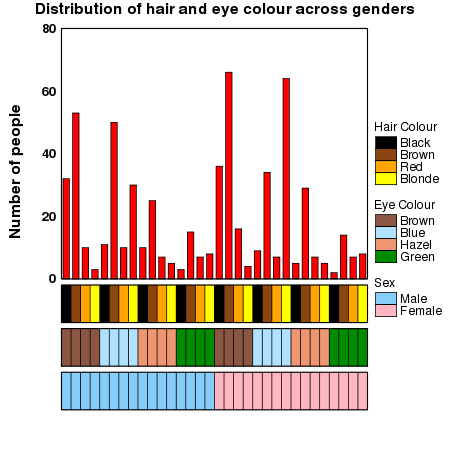
\includegraphics[width=70mm]{Figures/Multiplot_Ex1.png}
     \caption{Finished example 1 plot}
     \label{fig:picture}
  \end{center}
\end{figure}

\subsection{Example 2: Complex layout}

In this example we make a plot to convey gene expression using a more complex layout. This plot consists of two bar plots and two heatmaps. The heatmap takes up most of the figure and represents gene expression level changes in different samples. The top bar plot will represent the amount of sample used, and the side bar plot represents the importance of the gene. (Note that this example is not based upon real data.)

\begin{figure}[!ht]
  \begin{center}
     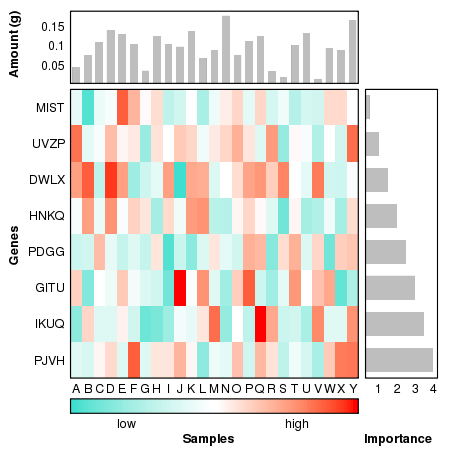
\includegraphics[width=80mm]{Figures/Multiplot_Ex2.png}
     \caption{Finished example 2 plot}
     \label{fig:picture}
  \end{center}
\end{figure}

\subsubsection{Setting up the data}

Data is generated for this example: 

\begin{verbatim}
set.seed(12345);

# main heatmap data
heatmap.data <- data.frame(
    a = rnorm(n = 25, mean = 0, sd = 0.75),
    b = rnorm(n = 25, mean = 0, sd = 0.75),
    c = rnorm(n = 25, mean = 0, sd = 0.75),
    d = rnorm(n = 25, mean = 0, sd = 0.75),
    e = rnorm(n = 25, mean = 0, sd = 0.75),
    f = rnorm(n = 25, mean = 0, sd = 0.75),
    g = rnorm(n = 25, mean = 0, sd = 0.75),
    h = rnorm(n = 25, mean = 0, sd = 0.75)
    );

# colourkey data
colorkey.data <- data.frame(
    x <- seq(-50,50,1)
    );

# top barplot data
top.barplot.data <- data.frame(
    x = rnorm(n = 25, mean = 2, sd = 0.75),
    y = seq(1,25,1)
    );
 
 # side barplot data
side.barplot.data <- data.frame(
    x = rnorm(n = 8, mean = 0, sd = 0.75),
    y = seq(1,8,1)
    );
\end{verbatim}

\subsubsection{Creating the main heatmap}

Here the heatmap used to display the expression level for each sample and gene is created. 

\begin{verbatim}
gene.expression.heatmap <- create.heatmap(
     x = heatmap.data,
     xaxis.tck = 0,
     yaxis.tck = 0,
     colourkey.cex = 1,
     
     # Don't want to cluster this heatmap
     clustering.method = "none",
     axes.lwd = 1,
     ylab.label = "y",
     xlab.label = "x",
     yaxis.fontface = 1,
     xaxis.fontface = 1,
     xlab.cex = 1,
     ylab.cex = 1,
     main.cex = 1,
     colour.scheme = c("red", "white", "turquoise")
     );
\end{verbatim}

\begin{figure}[!ht]
  \begin{center}
     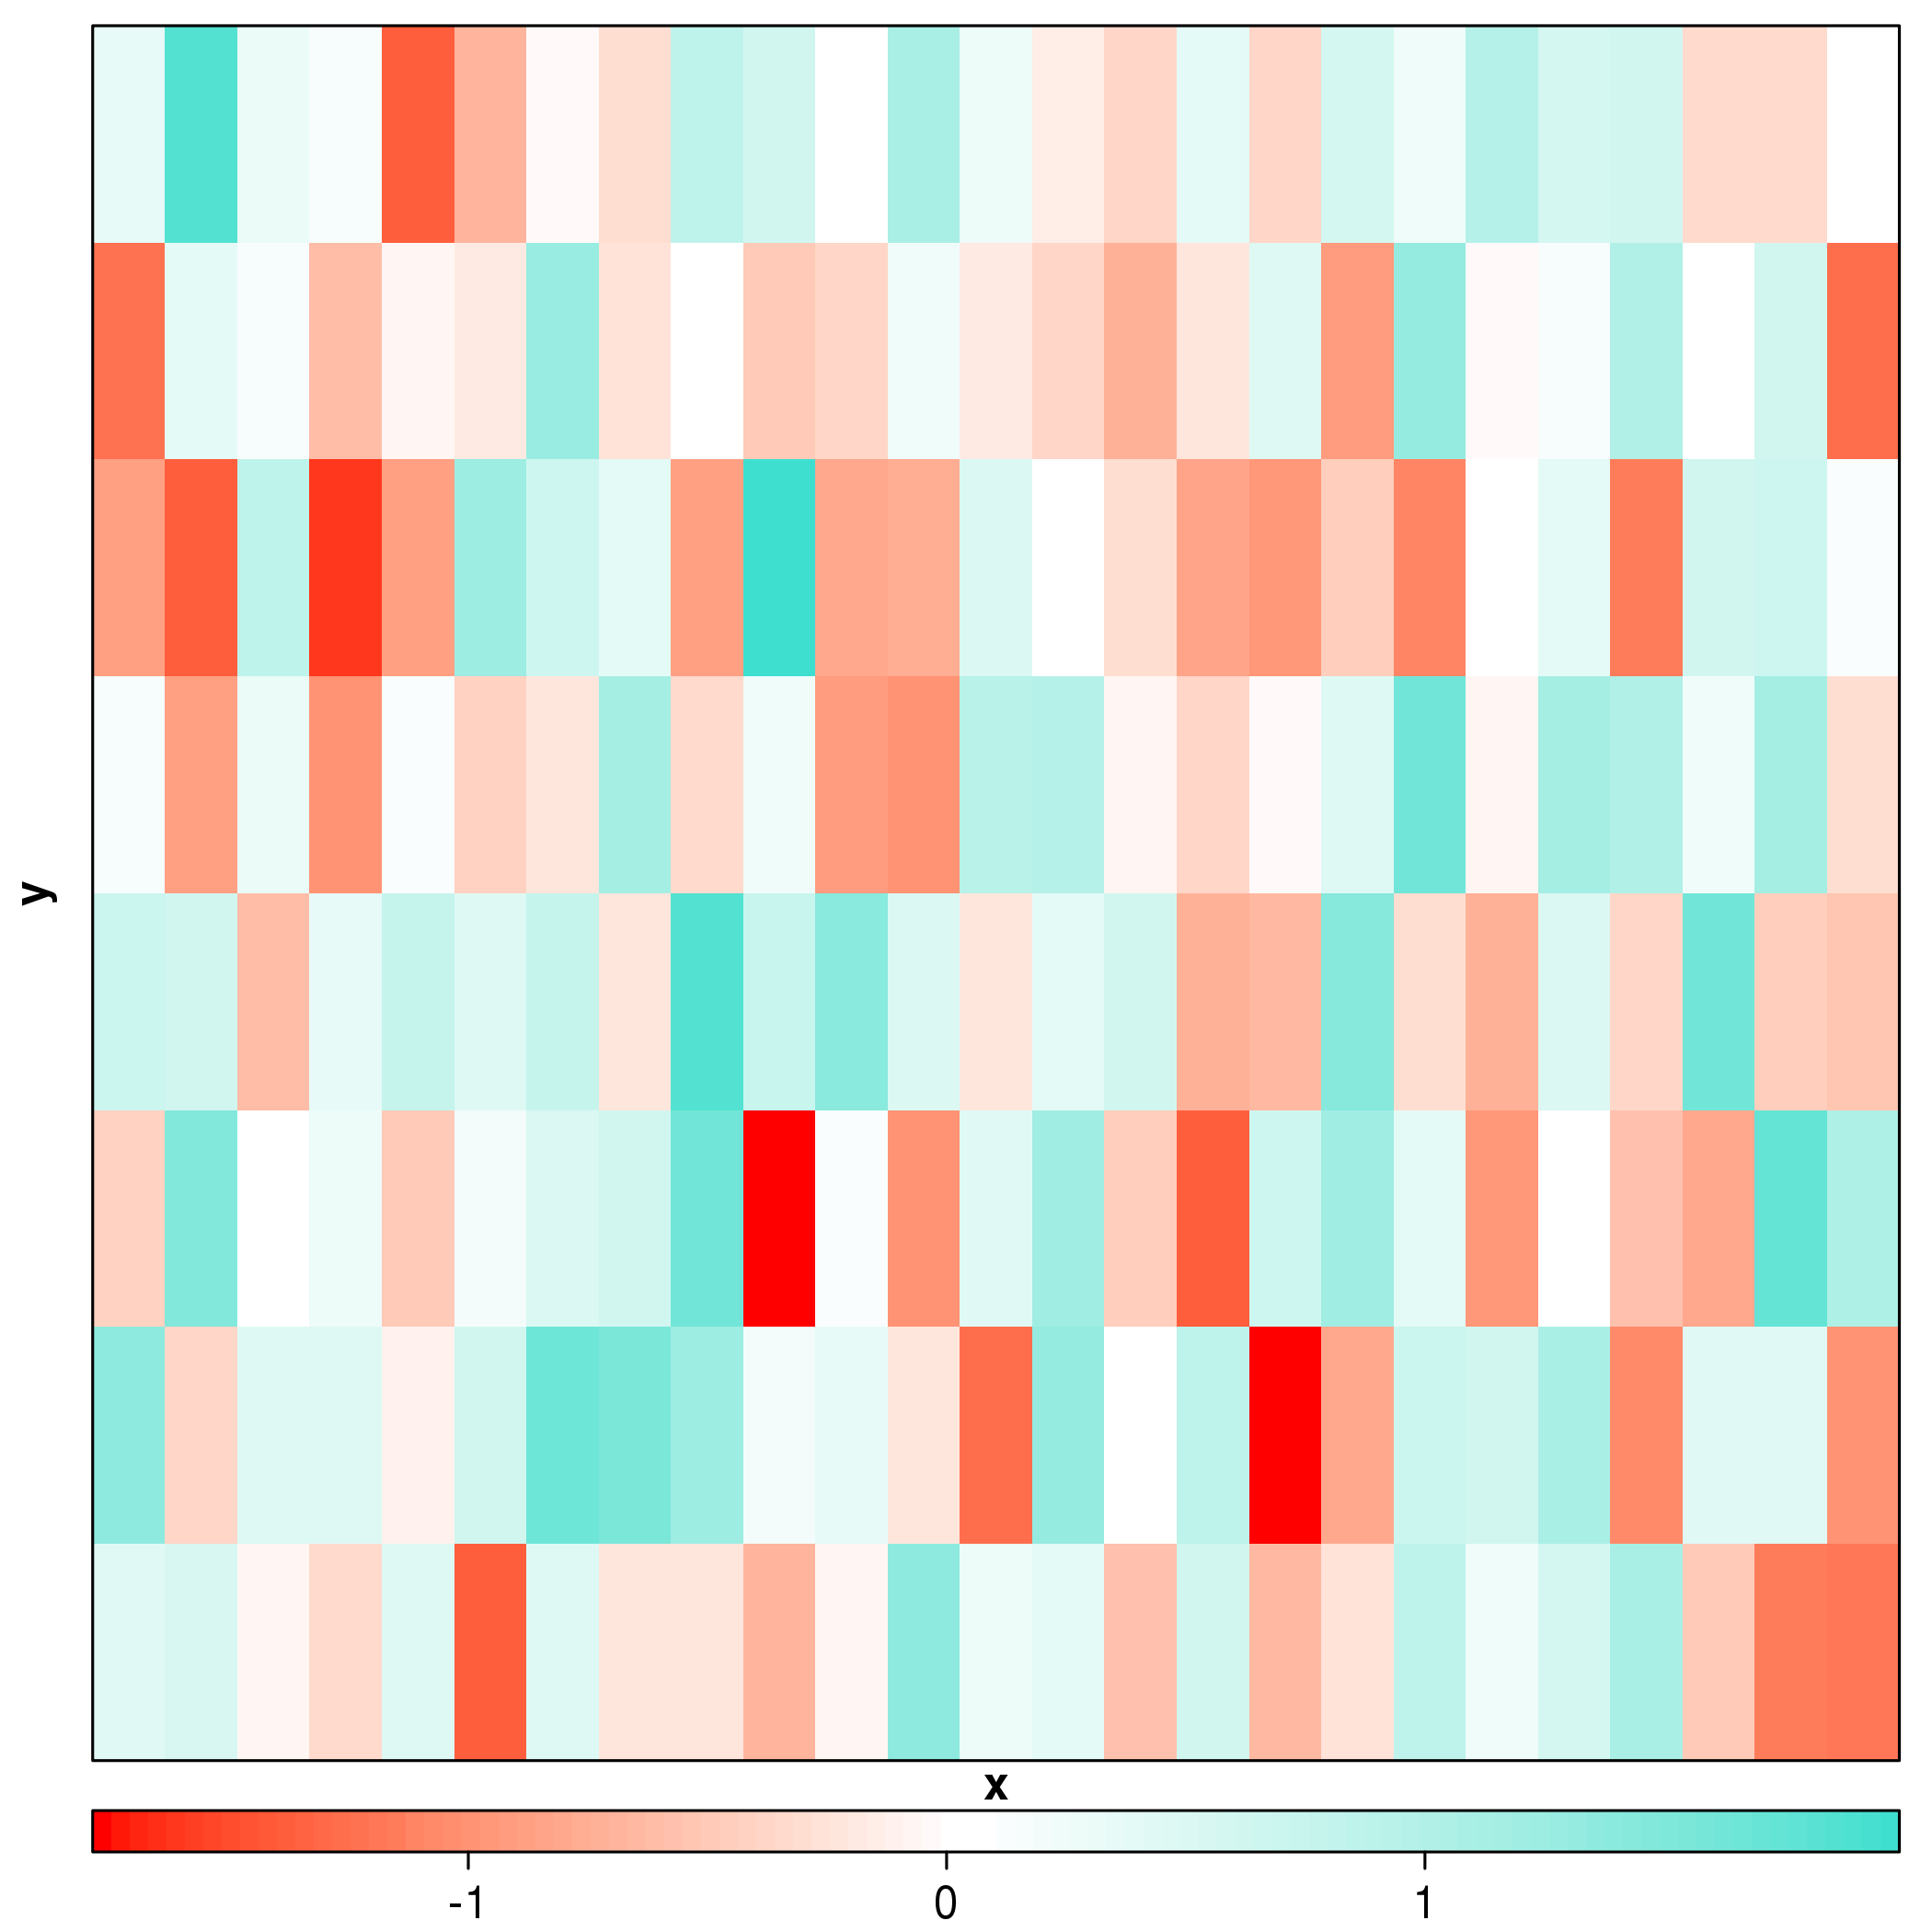
\includegraphics[height = 50mm]{Figures/ex2_heatmap.png}
     \caption{Main heatmap}
     \label{fig:picture}
  \end{center}
\end{figure}

\subsubsection{Creating the colourkey}

Here the colourkey for the main heatmap is created. It displays the same colours as the heatmap, as well as indicate what the colours represent.

\begin{verbatim}
key <- create.heatmap(
   x = colorkey.data,
   clustering.method = "none",
   scale.data = FALSE,
   # set the same colours as are in the heatmap
   colour.scheme = c("turquoise", "white", "red"),
   print.colour.key = FALSE,
   yaxis.tck = 0,
   xat = c(10, 90),
   xaxis.lab = c("low", "high"),
   xaxis.rot = 0,
   xaxis.cex = 2,
   height = 1
   );
\end{verbatim}

\begin{figure}[!ht]
  \begin{center}
     
\includegraphics[width=50mm]{Figures/ex2_colourkey.png}
     \caption{Main heatmap colourkey}
     \label{fig:picture}
  \end{center}
\end{figure}

\subsubsection{Creating the top bar plot}
The bar plot at the top of the plot representing the amount of sample is created. The bar plot will look very simple, but details will be added later when the create.multiplot function is called.

\begin{verbatim}
sample.barplot <- create.barplot(
     formula = x~y,
     data = top.barplot.data,
     
     # This will remove lines
     lwd = 0
     );
\end{verbatim}

\begin{figure}[!ht]
  \begin{center}
     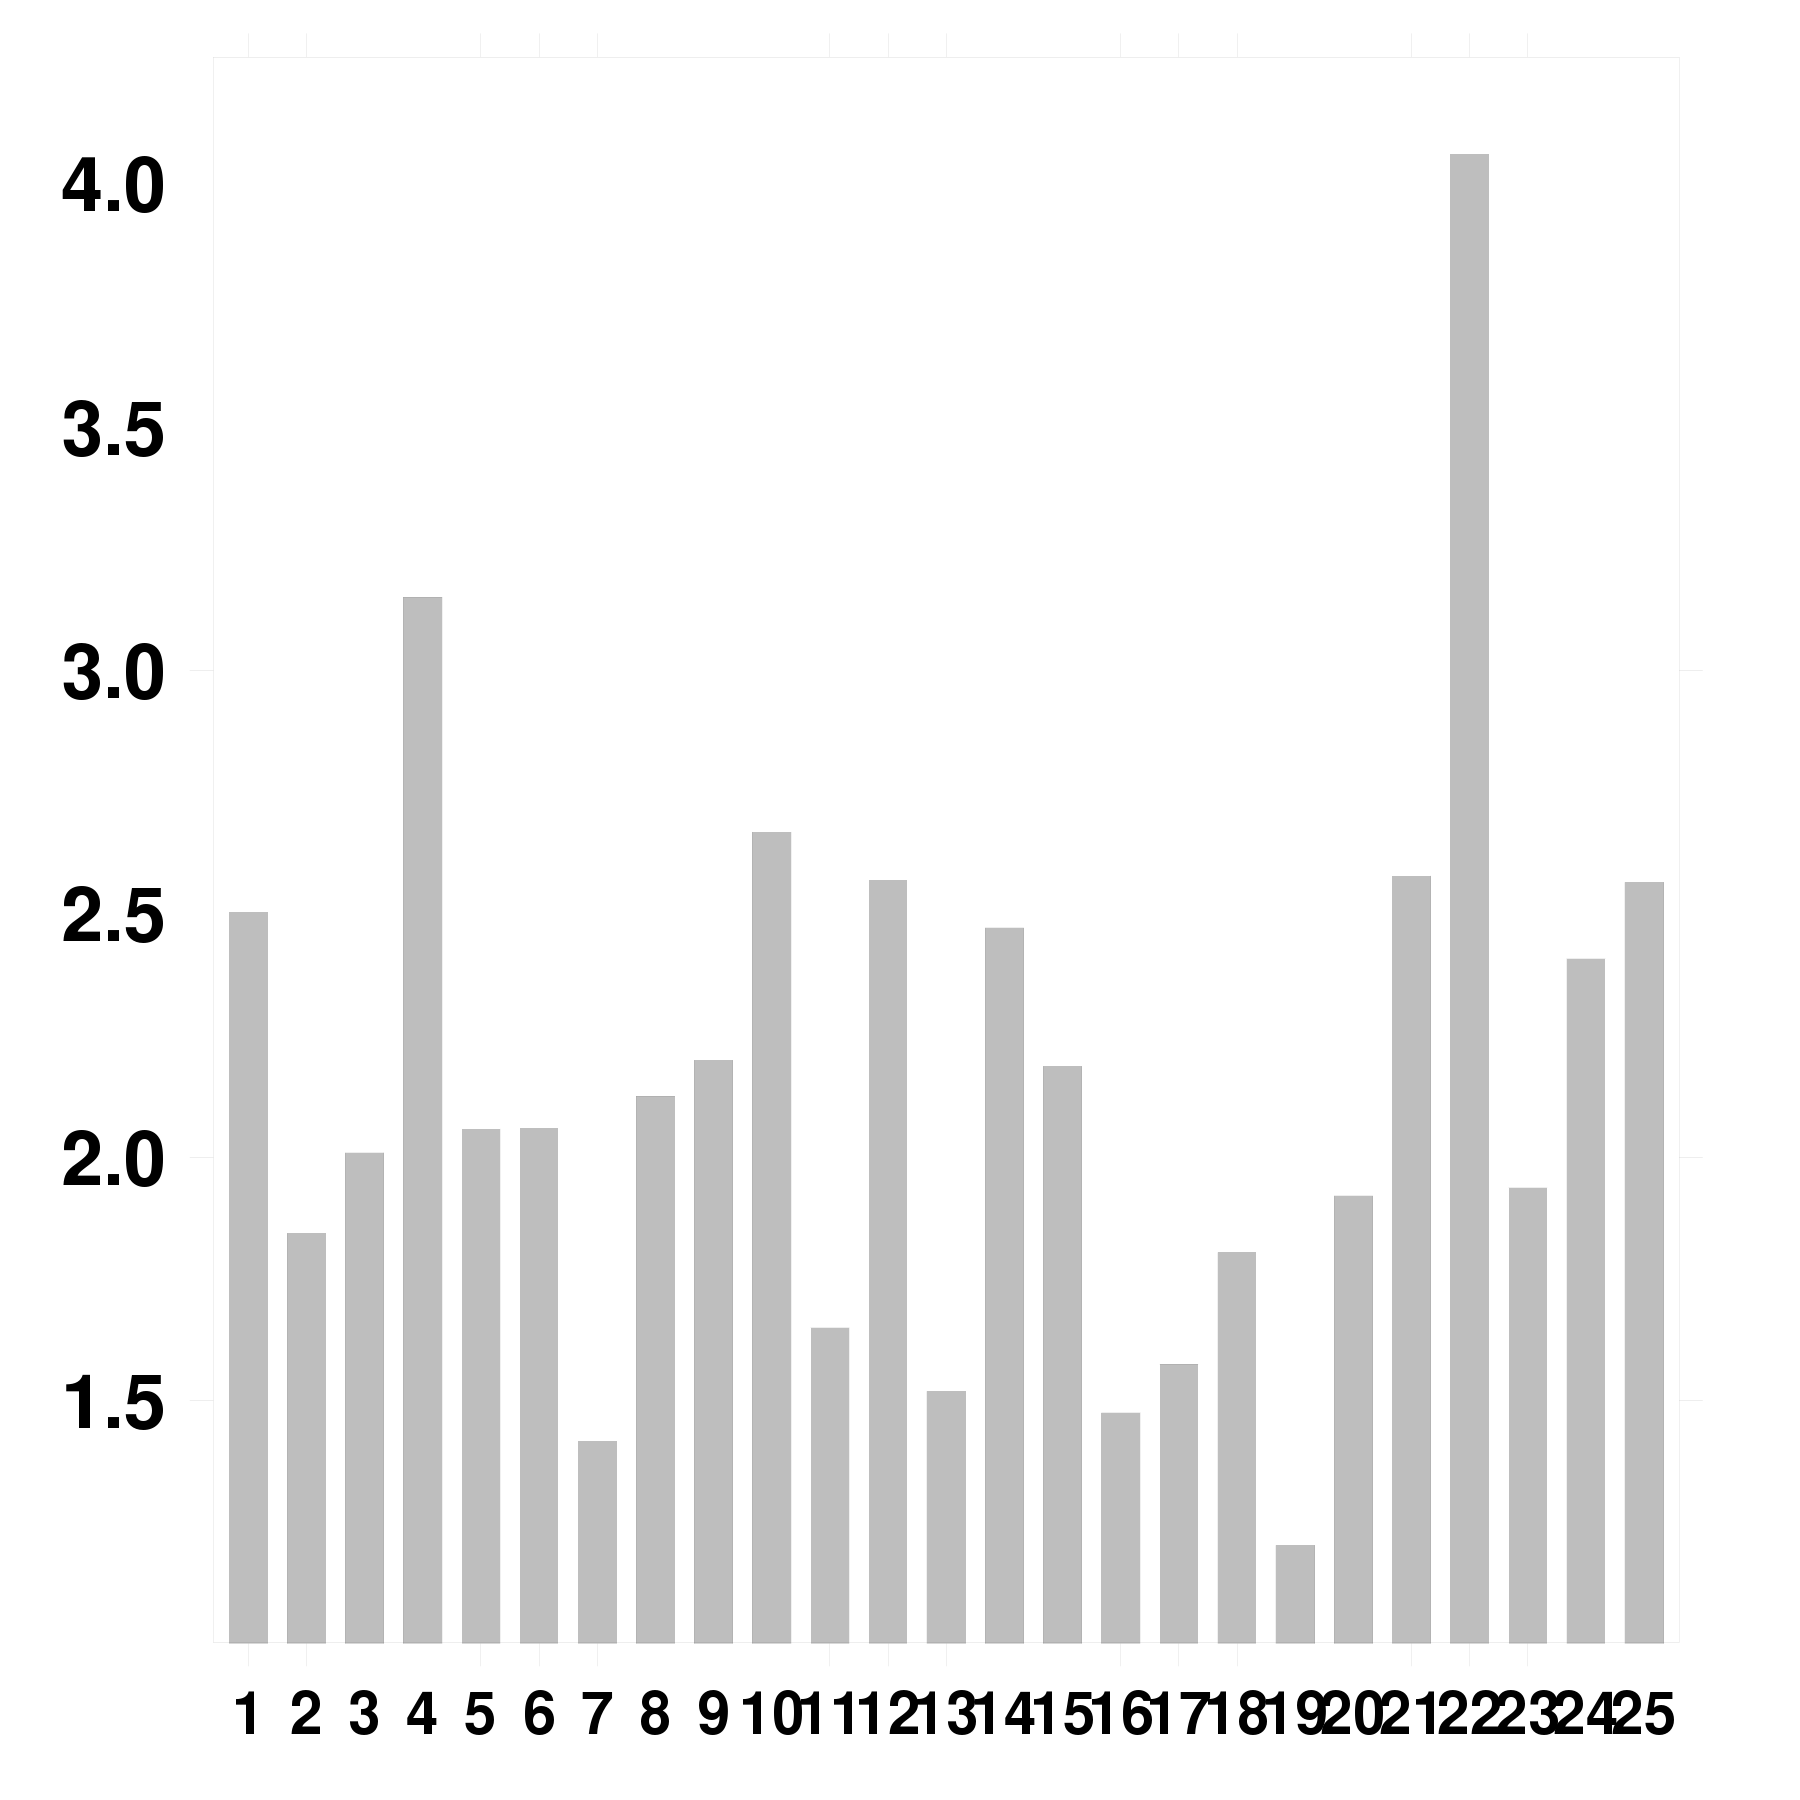
\includegraphics[width=50mm]{Figures/ex2_sample_barplot.png}
     \caption{Top bar plot}
     \label{fig:picture}
  \end{center}
\end{figure}

\subsubsection{Creating the side bar plot}

Here the side bar plot representing the importance of the gene is created. The bar plot will look very simple, but details will be added later when the create.multiplot function is called.

\begin{verbatim}
importance.barplot <- create.barplot(
     formula = x~y,
     data = side.barplot.data,
     lwd = 0,
     
     # The data here is sorted. 
     # Note that if real data was used, we would have to ensure that the corresponding heatmap rows were similarly sorted to match
     sample.order = "decreasing",
     plot.horizontal = TRUE
     );
\end{verbatim}

\begin{figure}[!ht]
  \begin{center}
     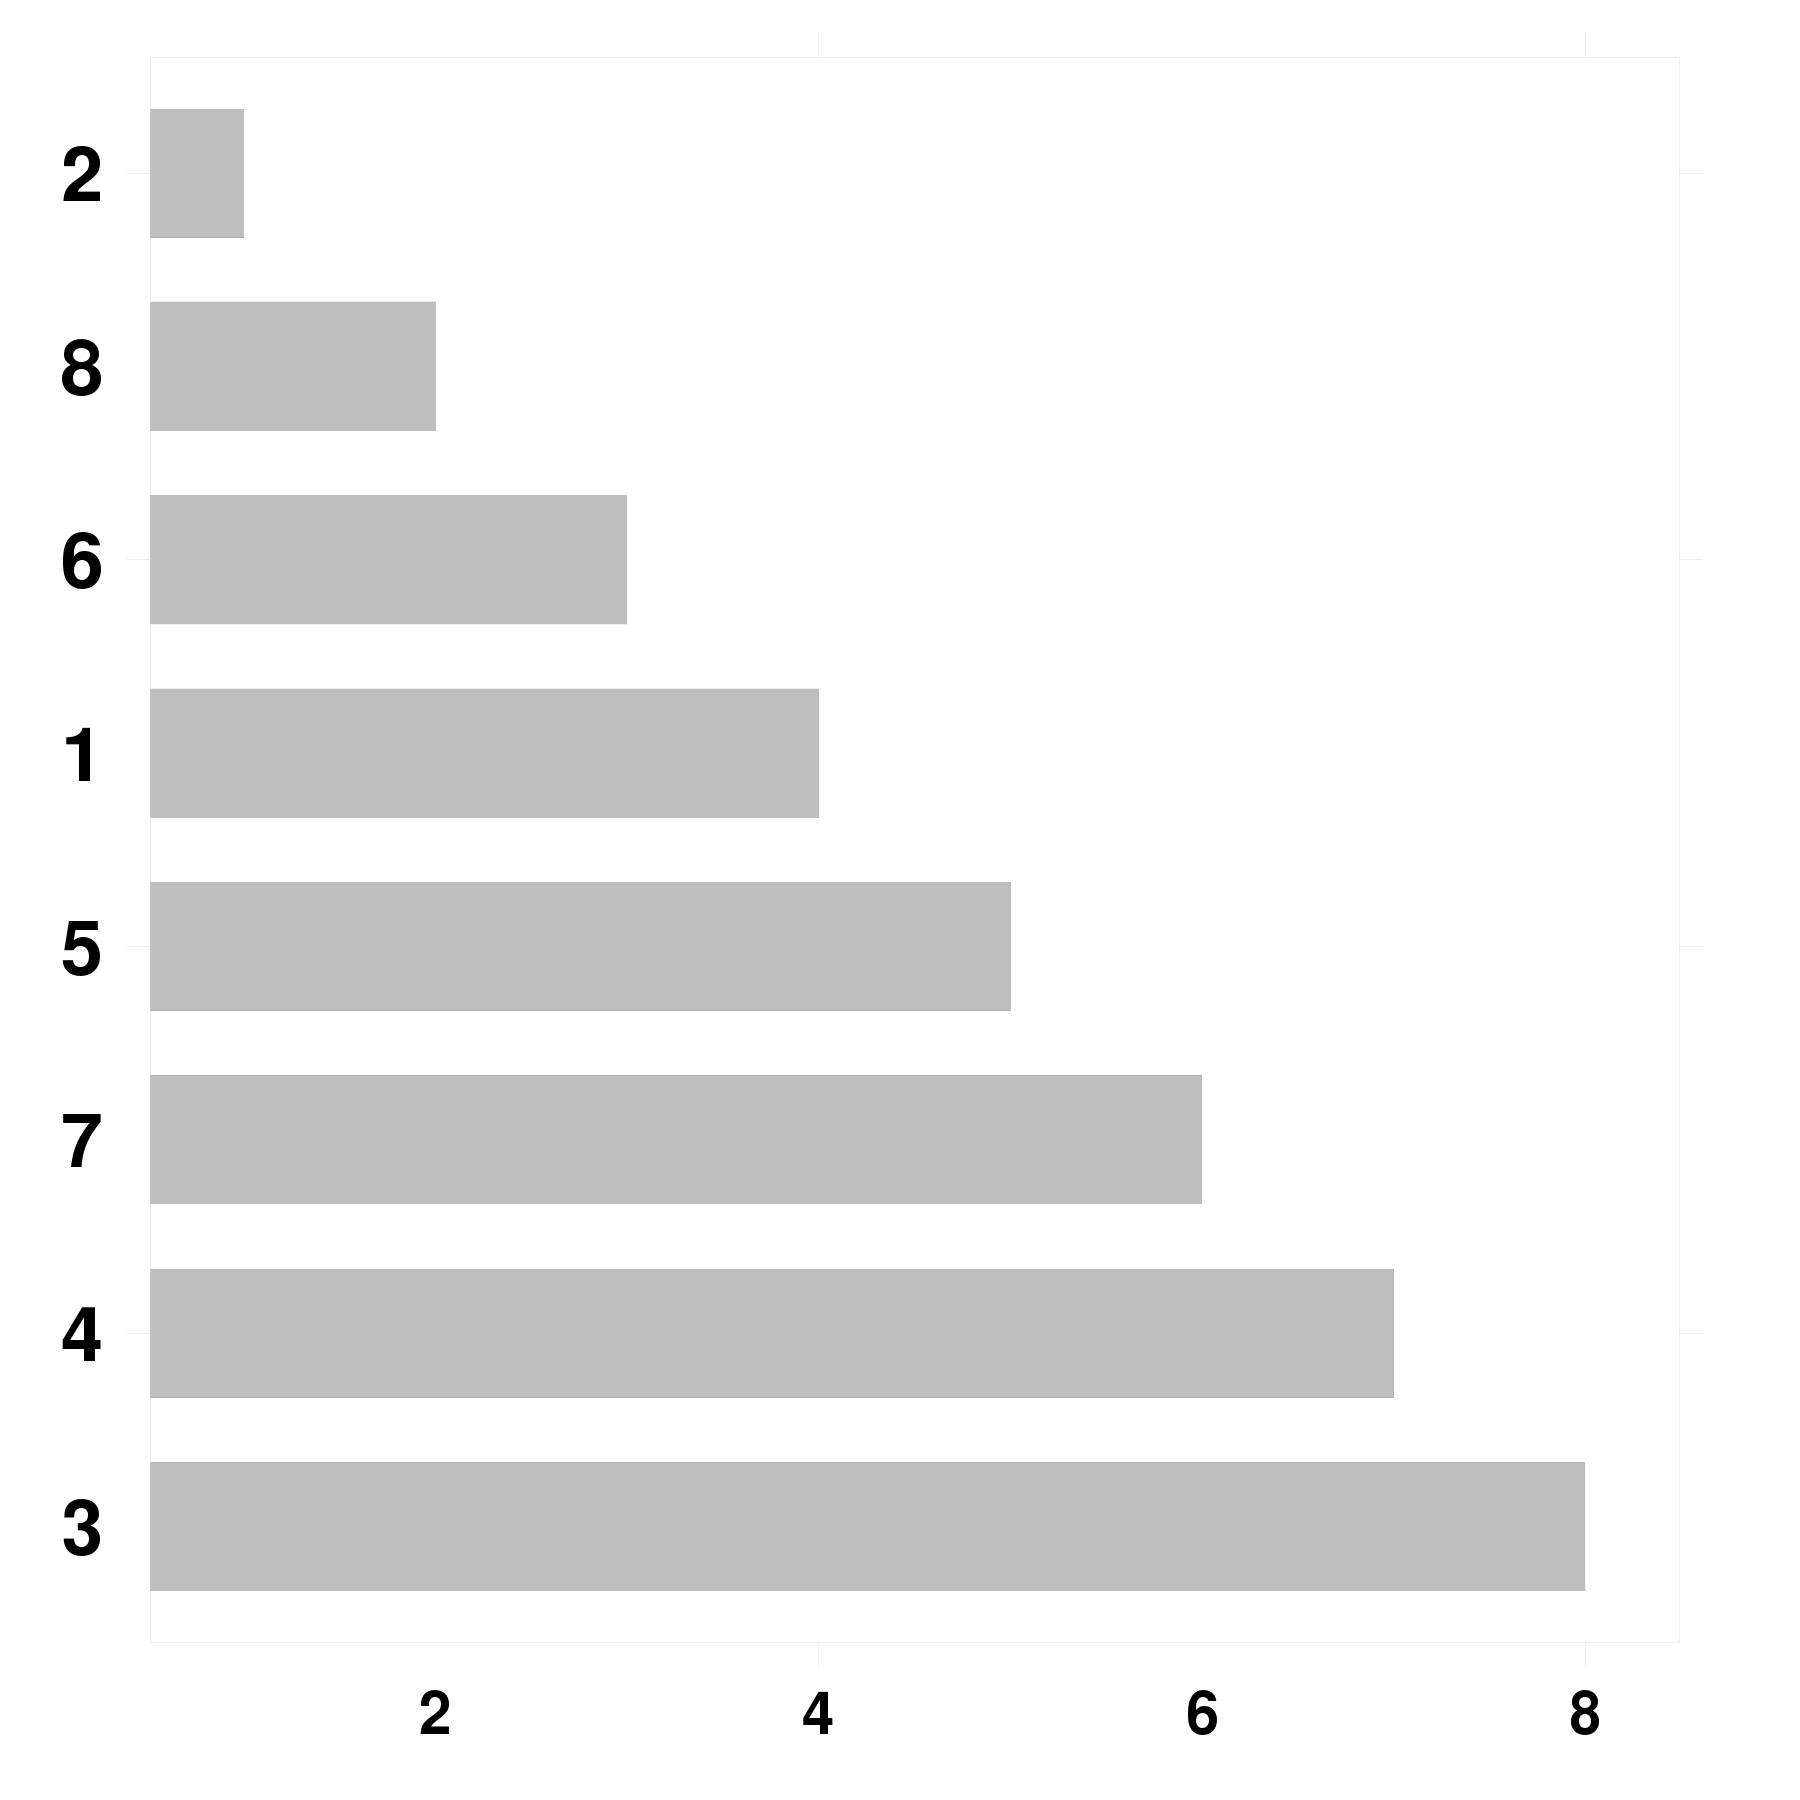
\includegraphics[width=50mm]{Figures/ex2_importance_barplot.png}
     \caption{Importance Bar Plot}
     \label{fig:picture}
  \end{center}
\end{figure}

\subsubsection{Creating the final figure}

The create.multiplot function is used to combine the plots. First consider the layout: this plot uses 3 rows of 2 columns and skips the bottom right plotting space. The bottom row contains just the colourkey, the middle row contains the main heatmap and the side bar plot, and the top row contains the top barplot. Below is a figure describing the layout; blue represents an area that a plot will appear there, red represents an area that is skipped, and yellow represents an unused area.

\begin{figure}[!ht]
  \begin{center}
     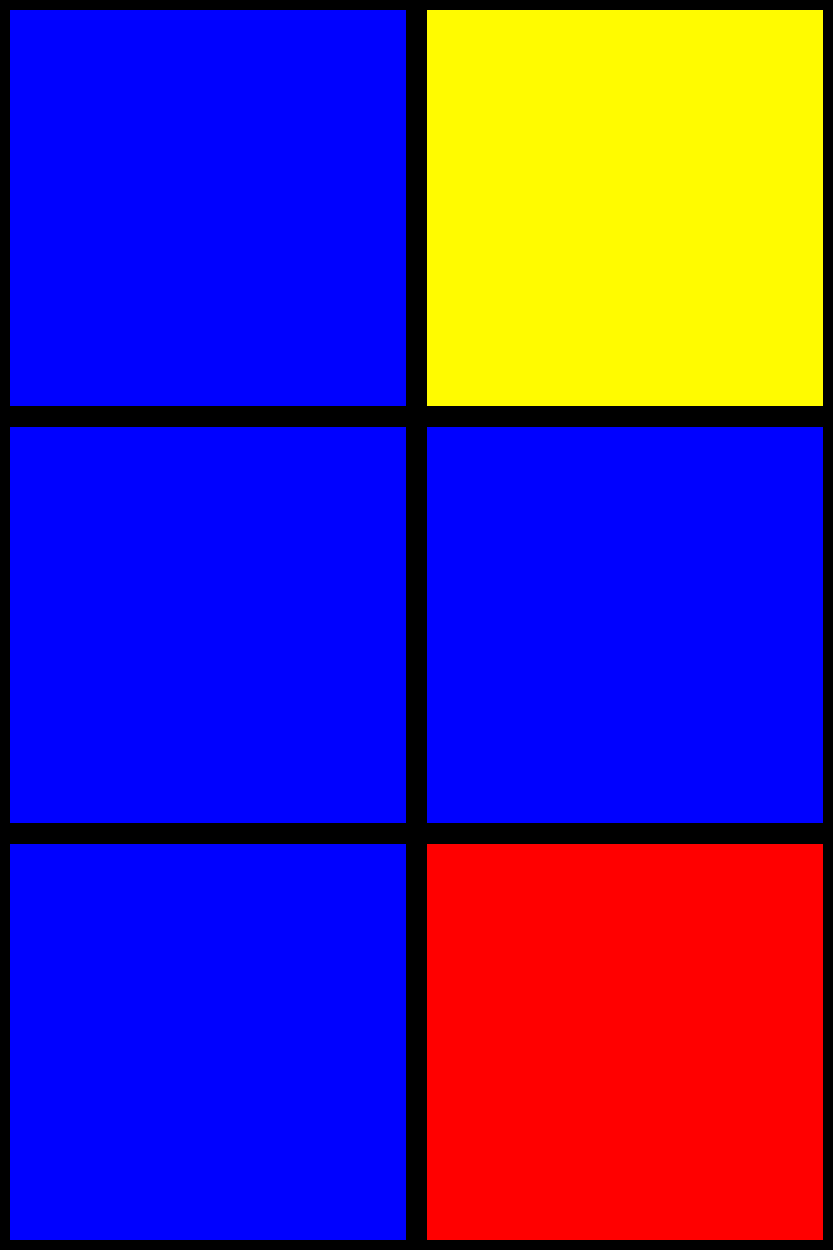
\includegraphics[width=25mm]{Figures/ex2_schematic.pdf}
     \caption{Plot layout}
     \label{fig:picture}
  \end{center}
\end{figure}

\begin{verbatim}
create.multiplot(
    # use the four plots we created earlier as the objects for the multiplot
    filename = "Multiplot_Ex2.png",
    plot.objects = list(key, gene.expression.heatmap, importance.barplot, sample.barplot),
    panel.heights = c(0.25, 1, 0.05),
    panel.widths = c(1, 0.25),
   
    # this is where we will specify how the plots layout will look
    # plot.layout specifies the number of rows and columns (3 rows, 2 columns)
    # layout.skip specifies which of the plots in the specification will be skipped
    # the skip specification starts at the bottom left, moves to the right and then up
    plot.layout = c(2, 3),
    layout.skip = c(FALSE, TRUE, FALSE, FALSE, FALSE, FALSE),
    xaxis.alternating = 0,
    yaxis.alternating = 0,
    xaxis.cex = 1,
    yaxis.cex = 1,
    xlab.cex = 1,
    ylab.cex = 1,

    # format labels (tabs are needed for proper spacing between labels)
    xlab.label = c("\t", "Samples", "\t", "    Importance"),
    ylab.label = c( "Amount (g)", "\t", "\t", "Genes", "\t", "\t"),
    ylab.padding = 6,
    xlab.to.xaxis.padding = 0,
    xaxis.lab = list(
        c("","low","", "","high", ""),
        LETTERS[1:25],
        seq(0,5,1),
        NULL
        ),
    yaxis.lab = list(
        NULL,
        replicate(8, paste(sample(LETTERS, 4, replace = TRUE), collapse = "")),
        NULL,
        seq(0,4,0.05)
        ),
    xspacing = -0.5,
    yspacing = c(0, -1),
    xaxis.fontface = 1,
    yaxis.fontface = 1
    );
\end{verbatim}

\begin{figure}[!ht]
  \begin{center}
     \includegraphics[width = 70mm]{Figures/Multiplot_Ex2.png}
     \caption{Finished Example 2 Plot}
     \label{fig:picture}
  \end{center}
\end{figure}

\subsection{Troubleshooting}
This section briefly outlines some issues that beginners may have with the multiplot function. 
\newline
\newline
1. The way that the plots are displayed according to the layout you specify may be confusing. The first plot you specify in plot.objects is going to be drawn at the bottom left most area for a plot and the ordering will then fill the plots to the right. After reaching the rightmost plot, the plots in the row above will begin to be drawn. 
\newline
\newline
2. A common mistake is that the amount of panel widths/heights must be a multiple of the number of plots. The warning will look like:

\begin{verbatim}
        1: In widths.x[pos.widths[[nm]]] <- widths.settings[[nm]] * widths.defaults[[nm]]$x : 
        number of items to replace is not a multiple of replacement length
        2: In widths.x[pos.widths[["panel"]]] <- widths.settings[["panel"]] *  :
        number of items to replace is not a multiple of replacement length
\end{verbatim}

This may cause the plots to not look as you intend, but is easily fixed by ensuring that your panel.widths and panel.heights parameters are multiples of the number of plots that can be plotted. For example, if your layout has 2 rows and 3 columns, the panel.heights parameter can have 2 inputs, and the panel.widths parameter can have 3 inputs.

\section{Other Functions}
The BL.plotting.general package contains a number of non-plotting functions which are included to assist in the plot-generation process. 

\subsection{Colours}
There are number of functions to help choose colours for plotting:
\begin{itemize}
\item \texttt{default.colours} provides a number of pre-made colour palettes to use
\item \texttt{force.colour.scheme} similarly provides colour palettes, but for specific use-cases
\item \texttt{colour.gradient} generates sequential colour schemes
\item \texttt{display.colours} gives a preview of a colour scheme along with grey scale values and colour names
\end{itemize}

The available generic colour schemes can be previewed simply using the \verb|display.colours| function:
\begin{verbatim}
# displays the pastel colour scheme
display.colours(default.colours(12, palette.type = "pastel"));

# displays the spiral.dusk colour scheme
display.colours(default.colours(5, palette.type = "spiral.dusk"));

# displays the case-specific biomolecule colour scheme
biomolecule_names <- c("DNA", "RNA", "Protein", "Carbohydrate", "Lipid");
display.colours(force.colour.scheme(biomolecule_names, "biomolecule"), biomolecule_names);
\end{verbatim}

The full range of colour schemes available is described in the documentation of the \verb|default.colours| and \verb|force.colour.scheme| functions.

The spiral.sunrise, spiral.dusk, etc colour schemes were created by ``spiralling'' through the colour wheel, varying the hue, saturation, and value of the colours to achieve a greater perceptual difference \cite{rainbow} \cite{wong2}. 

\subsection{Legends}
\begin{itemize}
\item \texttt{legend.grob} and \texttt{covariates.grob} create grob objects for legends and covariates respectively
\item \texttt{create.colourkey} is useful for adding colourkeys to multiplots
\item \texttt{get.corr.key} creates correlation key legends to be added to plots
\end{itemize}

\subsection{Text}
\begin{itemize}
\item \texttt{append.footnote} adds text to plots
\item \texttt{scientific.notation} function formats numbers into scientific notation
\item \texttt{display.statistical.result} function uses this to display statistical results in plots
\item \texttt{get.line.breaks} is used in the specific case of placing indices in heatmaps
\end{itemize}

\subsection{Private}
Other functions are called by plotting functions but are not intended for use by end-users: 
\begin{verbatim}
generate.at.final, get.defaults, write.metadata, write.plot
\end{verbatim}

\section{Designing figures}
Before creating figures, it is important to know something about design. Terrible design will miscommunicate data, whereas excellent design will guide viewers to understand the data\cite{tufte}. 

\subsection{Typography}
Typography is the art of arranging type to make written words understandable. This encompasses decisions related to which typeface to use, at which size, with what line spacing, and more. 

When it comes to choosing fonts for a figure, it is advisable to use no more than one or two fonts. The distinction between a typeface and a font is often confused: a typeface is Arial, which is made up of a number of fonts, such as Arial bold, Arial roman, Arial italic, and other such fonts \cite{wong-type}. Thus, when selecting which fonts to use in a figure, one option is to use Arial roman for most text, and Arial bold for headers.

Another options for selecting different fonts is to choose very different fonts. This can be achieved by combining a serif and sans serif font with different font size, colour, boldness, etc \cite{williams}.

Typefaces can be divided into two classes: serif and \textsf{sans serif}. A serif is a small mark found at the tips of letter forms. Serif fonts have serifs (such as Times New Roman), while \textsf{sans serif} fonts do not have serifs (such as Arial). There are mixed opinions as to which kind is advisable for which occasion.

For figures, I would advise using common fonts, such as Arial. Unusual fonts may give unintended impressions, and has the danger of distracting viewers from the message, especially when the vast majority of figures use very standard fonts. This is enforced by journals, which often have figure guidelines restricting font choice. 

If there is sufficient cause to use an unusual font, ensure that the chosen font is legible and appropriate for the use-case. 

\subsection{Principles of design}
The following principles of design are concepts to keep in mind when arranging elements of a design: \cite{williams}
\begin{itemize}
\item Contrast: used to attract the eye and organize the composition
\item Repetition: creates unity and consistency
\item Alignment: adds visual connection between elements and helps to unify and organize
\item Proximity: group related items helps organization and movement
\end{itemize}

\begin{figure}[!ht]
  \begin{center}
     \includegraphics[width=50mm]{Figures/Multiplot_Ex2.png}
     \caption{Multiplot example}
  \end{center}
\end{figure}

Take this figure as an example. The bright red cells in the heatmap attract the eye first: they contrast the white and turquoise. This highlights the genes and samples with a high expression change. This bright red is repeated in the colour key underneath the heatmap, as well as in varying degrees of saturation throughout the heatmap to unify the figure. The surrounding barplots and colour key are properly aligned to the borders of the heatmap, and each barplot is in close proximity to the row or column it is associated with. 

When designing a layout, it is important to understand which elements of the composition are most important: what \textit{should} a viewer notice first? Good layout controls how the viewer's eye moves around the page. Therefore, the most important elements should stand out the most. This can be done by varying the colour, size, shape, and more. In addition, if a design is divided into thirds in both directions, the intersections of the dividing lines is where focal points should be located. This is called the rule of thirds \cite{wong3}.

\subsection{Understanding colour}
Colour is a highly relative medium. Someone might say that red is an `angry' colour. Another person seeing the same colour may believe instead that red is associated with being `lucky'. There is no consensus on what a colour means. 

\subsubsection{Colour theory}
Colour can be described in three ways:
\begin{itemize}
\item Hue is what the colour is called, for example `red'
\item Saturation is how vibrant the colour is: `dull red' versus `bright red'
\item Value is how light or dark the colour is: `light red' versus `dark red'
\end{itemize}

\begin{figure}[!ht]
  \begin{center}
     \includegraphics[width=50mm]{Figures/colour_wheel.png}
     \caption{Colour wheel}
  \end{center}
\end{figure}

The colour wheel is a way of arranging colours such that primary colours are equidistant, and the result of their mixing fills in the in-between segments (which are called the secondary and tertiary colours). This colour wheel shown is the one commonly used by artists, where the primary colours are red, yellow, and blue. 

Red, orange, and yellow are considered the `warm' colours, while green, blue, and purple are the `cool' colours. The warm colours are thought to attract more attention (with red being the most attention-grabbing colour), while the cool colours tend to visually recede. This means that if equal amounts of warm and cool colours are in a design, the warm colours will dominate. This applies to data visualization because of two equal areas of a plot are coloured red and green, the red areas will appear larger \cite{tedford} - although this only appears to be the case for high-saturation colours \cite{cleveland-colour-illusion}

Complementary colours are colours which are placed at opposite ends of the colour wheel (for example: red and green). These colour combinations achieve the highest hue-based contrast. A triad of colours is made up of three colours which are equidistant on the colour wheel. A double complement is composed of two sets of complementary colours. Analogous colours neighbour each other on the colour wheel. 

\subsubsection{Colour models}
There are different ways of generating colour, and consequently colours displayed on different mediums often do not appear the same. For example, a colour scheme might be easily distinguishable on a computer screen, but not when printed. 

Computer monitors generate colours using the RGB colour model, which is based on light (primary colours are red, green, and blue). In contrast, printers generate colours using the CMYK colour model, which is made with ink (primary colours are cyan, magenta, and yellow) \cite{silva}. The important thing to note is that the colours made in RGB and the colours made in CMYK may not appear the same. RGB creates a more vibrant spectrum of colours than CMYK: this is why printed material often appears duller than on a computer monitor. Therefore, if you expect your figure to be reproduced in print, use the CMYK colour model to have a more accurate idea of what the final image will look like.

CMYK and RGB are device-dependent colour models. This means that a colour specified using these colour models may appear different when created using different devices \cite{silva}. Some software can convert CMYK colours to RGB and vice versa, however different software use different algorithms to do this conversion \cite{brewer-colour}. The result is that a single colour, converted to a different colour model using two different software will produce two different colours. The same problem can be found when using different printers and even across operating systems with different monitor calibration \cite{brewer-colour}. 

\subsubsection{Colour blindness}
Colour blindness is a decreased ability to distinguish colours, which affects a significant percentage of the population. The most common forms affect a person's ability to distinguish red and green.

When choosing colours, it is good practice to accommodate colour blind individuals. There are a number of ways to do this: one method is by not relying on colour hue alone, but also colour value and other elements. For example, a scatter plot might use different plotting characters in addition to different coloured dots. 

Another option is to avoid colour schemes which mix colours with components of red and green. Alternatives include red-turquoise and green-magenta colour combinations \cite{wong4}.

Using software to simulate colour blindness can be a good test of whether or not a given figure will be challenging to interpret for colour blind individuals \cite{wong4}.

Choosing colour schemes which are greyscale-compatible is desirable both for people with colourblindness and for when figures are reproduced in black and white. There are two main ways to ensure a figure is decipherable in greyscale and it is advisable to use both. The first method is by choosing colours with large differences in value (lightness and darkness). This with create a variety of greys, whereas if all colours have the same value, they will appear to be the same grey. The second method is by varying the plotting characters or line types. For example, a scatterplot might use circles and triangles to divide different groups in addition to differently coloured points. 

\subsubsection{Simultaneous contrast}
The perception of colour varies based on its surroundings. If a person stares intently at a red square for a time, then suddenly shifts his gaze to a white square, he will for a moment perceive green instead of red. This is called simultaneous contrast: the phenomenon when colours influence the perception of other colours to have greater contrast \cite{albers}. 

This affects both value and hue. A blue surrounded by grey will cause the grey to appear more like a yellowish grey. The consequence is that there is some danger with using complementary colours: for example, if a figure contains a mix of blues and yellow of varying values, a light yellow surrounding a blue may cause it to appear darker and more saturated, such that it may be confused with the next darkest blue in the colour scheme \cite{brewers-sim}. 

Therefore, when selecting colour schemes which are used in mixed arrangements, avoid complementary colours. This also avoids a perceptual ``vibration'' which occurs when complementary colours of similar values are neighbours \cite{brewers-sim}.

\subsubsection{Data-appropriate}
Use appropriate colours for the data at hand. For example, if the data progresses from low to high values, it may be intuitively visualized using a sequential colour scheme, which uses value differences. If the data increases in two directions (such as in the positive and negative directions), use a diverging colour scheme. If there is no intuitive magnitude differences in the data, as is the case with nominal and categorial data, use a qualitative scheme, which relies primarily on differences in hue \cite{brewer-colour}.

The rainbow colour map is often used in visualizations for sequential data, however it is not a good choice \cite{rainbow}. Although the colours in a rainbow \textit{are} ordered based on wavelength of light, this ordering is not perceptual (unlike value-based ordering). In addition, this colour scheme progresses with uneven perceptual steps, as each hue change is a sharp change, while the progression within a hue is comparatively slow. This colour scheme should be avoided.

Sometimes the data suggests which colour should be used. For example, if a figure compared blue eyes and green eyes, the data points might be coloured blue and green. 

In some fields of study, colour conventions are in place. These convention can be used to help make data quickly recognizable to viewers \cite{rheingans}, and at the very least, colour schemes should not reverse conventions, as this would likely lead to confusion. 

Whether colour is even necessary at all should be considered \cite{wong-avoid-colour}. Colour is a relative medium, difficult to interpret accurately, poses problems to people with colour blindness and may result in loss of clarity when images are reproduced in greyscale. It is easy to default to using colour in figures because of its aesthetic value, but it important to consider whether or not colour is the most effective method of communicating data.

\subsection{File type}
There are multiple ways of classifying file types. Understanding the distinctions will help with selecting the appropriate file type.

\subsubsection{Raster vs. vector}
Images can either be raster (also known as bitmap) or vector. Raster images are encoded as pixels, which is why they appear pixelated when zoomed in. On the other hand, vector images are represented by mathematical expressions, which means that they can be infinitely scaled without losing resolution. 

Photographs are raster images. In order to print a large raster image, the image must have a high resolution (which increases the file size). 

Logos are often made to be vector images. This is because they expect to be reproduced at different sizes. 

\subsubsection{Image format}
There are many different kinds of image formats available, which will produce either raster or vector images. Some examples of vector images are PDFs and SVGs. Some common bitmap examples include JPEGs, TIFFs, PNGs, and GIFs. 

Bitmap images can be compressed using either lossless or lossy algorithms. Lossless algorithms decrease file sizes without compromising the quality of the image, whereas lossy algorithms decrease file size by sacrificing image quality. However, lossy algorithms are often able to create a smaller image size. JPEGs generally use a lossy compression algorithm. This means that each time you edit and save a JPEG image, some of the image quality is lost. 

A second consideration is what type of colour mode is supported. JPEG, PNG, and GIF use the RGB colour model, which is how colour is generated on digital displays. If an image is intended to be printed, the TIFF format also supports the CMYK mode.

Sometimes an image is very simple and uses very few colours. GIFs are small files and only support 256 colours, making them ideal for these instances.

Sorted by increasing file size:
\begin{center}
\begin{tabular}{l l l l }
\hline
File type & Compression & Mode & Colours \\
\hline
GIF & Lossless & RGB & 256 \\
JPEG &  Lossy & RGB & millions\\
PNG &Lossless & RGB &  millions \\
TIFF & Lossless & RGB, CMYK, etc & millions \\
\end{tabular}
\end{center}
\bigskip
In summary: use TIFFs for print, use PNGs for smaller file size without quality loss, use JPEGs if some quality loss is acceptable, and use GIFs when only few colours are needed.

The file type used by BL.plotting.general is determined by adding the extension to the file name. If no extension is specified, the package defaults to creating TIFF files.

\subsection{Resolution}
Image resolution is relevant to raster images which are not scalable. Pixel resolution is the type most commonly referred to when image resolution. This refers to the number of pixels in an inch, also called dots per inch (dpi) and describes the amount of detail an image holds.

Therefore, the image resolution is related to (but not the same as) the image size. If an image has a resolution of 72 dpi, this means that 72 pixels are stored in each inch. If the image is enlarged, the resolution will decrease because the pixel size apparently increases. Conversely, if the image is shrunken, there is option of increasing the resolution.

Different use-cases require different resolutions. Digital displays require lower resolutions than print displays. Most computer monitors are able to display a maximum of 72 dpi, which means that even if an image has a higher resolution, the display will only display a maximum of 72 dpi. 

Standard print resolution is often cited as 300 dpi. However, line art and text often need higher resolution to be clear. Journals may specify what resolution is required for figures. Bl.plotting.general defaults to producing high resolution images of 1000 dpi or greater.

\section{Figure creation reviewed}
Figure creation begins with understanding the data. The second step is designing the figure. Then the figure is created. Finally, the figure is assessed and improved.

Imagine a dataset comprising of two groups of subjects. One group runs for one mile, and the other group takes a nap. The heart rate for each subject is measured. How could this data be displayed? 

One option is to plot each data point on a scatterplot. The two groups could be distinguished by colour and plotting character. Another option is to use the distribution of heart rates and create two boxplots. There are many ways of showing the same data, and depending on what the intended message is, different methods may be more appropriate.

Plots in BL.plotting.general are created using a single function call. Depending on the function, mandatory parameters may be \verb|formula|, \verb|data| and/or \verb|x|. These parameters are used to indicate the data to be plotted and which variables to display.

Additional parameters may be used to adjust font sizes, add background shading, change colour schemes, and more. These parameters are optional and used for customization. The full range of parameters available is conveniently viewable on the BL.plotting.general API, together with extended example code of parameter usage.

Once a figure is made, it should be reproduced in its expected display format. For example, if a figure is expected to be printed in a journal, it should be assessed in a print format, and at the expected size. This allows viewers to check font legibility, colour differences, and other subtleties that may otherwise go unnoticed on screens.

\section{Resources}
Further information on the BL.plotting.general package can be found at  http://labs.oicr.on.ca/boutros-lab/software/bl.plotting.general.

\begin{thebibliography}{1}
\bibitem{Anscombe}
F.J. Anscombe, Graphics in Statistical Analysis. The American Statistician 27, 17-21 (1973).

\bibitem{wong-dataexploration}
Noam Shoresh \& Bang Wong, Data exploration. Nature Methods 9, 5 (2012).

\bibitem{wong1}
Bang Wong, Design of data figures. Nature Methods 7, 665 (2010).

\bibitem{cleveland}
William S. Cleveland \& Robert McGill, Graphical Perception and Graphical Methods for Analyzing Scientific Data. Science 229, 828-833 (1985).

\bibitem{tufte}
Edward R. Tufte, The Visual Display of Quantitative Information. Graphics Press, Cheshire, Connecticut (2001).

\bibitem{lattice}
Sarkar, Deepayan (2008) Lattice: Multivariate Data Visualization with R, Springer.  ISBN: 978-0-387-75968-5 URL: http://lmdvr.r-forge.r-project.org/

\bibitem{cleveland-scatter}
William S. Cleveland, Persi Diaconis \& Robert McGill, Variables on Scatterplots Look More Highly Correlated When the Scales Are Increased. Science 216, 1138-1141 (1982).

\bibitem{streit}
Marc Streit \& Nils Gehlenborg, Bar charts and box plots. Nature Methods 11, 117 (2014).

\bibitem{brewer-colour}
Mark Harrower \& Cynthia A. Brewer, ColorBrewer.org: An Online Tool for Selecting Colour Schemes for Maps. The Cartographic Journal 40, 27-37 (2003).

\bibitem{rheingans}
Penny Rheingans, Task-based Color Scale Design. In: Proceedings of the SPIE--28th AIPR Workshop: 3D Visualization for Data Exploration and Decision Making. 3905, 35-43 (2000).

\bibitem{rainbow}
David Borland \& Russell M. Taylor II, Rainbow Color Map (Still) Considered Harmful. IEEE Computer Graphics and Applications 27, 14-17 (2007).

\bibitem{Krzywinski}
Martin Krzywinski \& Naomi Altman, Visualizing samples with box plots. Nature Methods 11, 119-120 (2014).

\bibitem{wong2}
Bang Wong, Color coding. Nature Methods 7, 573 (2010).

\bibitem{wong-type}
Bang Wong, Typography. Nature Methods 8, 277 (2011).

\bibitem{williams}
Robin Williams, The Non-Designer's Design Book, 3rd ed. Peachpit Press, Berkeley, California (2008).

\bibitem{wong3}
Bang Wong, Layout. Nature Methods 8, 783 (2011).

\bibitem{tedford}
W. H. Tedford Jr., S. L. Bergquist \& W. E. Flynn, The Size-Color Illusion. The Journal of General Psychology 97, 145-149 (1977).

\bibitem{cleveland-colour-illusion}
William S. Cleveland \& Robert McGill, A Color-Caused Optical Illusion on a Statistical Graph. The American Statistician. 37, 101-105 (1983).

\bibitem{silva}
Samuel Silva, Beatriz Sousa Santos \& Joaquim Madeira, Using color in visualization: A survey. Computers \& Graphics 35, 320-333 (2011).

\bibitem{albers}
Josef Albers, Interaction of Color. Yale University Press, New Haven \& London (1963).

\bibitem{brewers-sim}
Cynthia A. Brewer, Guidelines for Selecting Colors for Diverging Schemes on Maps. The Cartographic Journal 22, 79-86 (1996).

\bibitem{wong4}
Bang Wong, Color blindness. Nature Methods 8, 441 (2011).

\bibitem{wong-avoid-colour}
Bang Wong, Avoiding color. Nature Methods 8, 525 (2011).

\end{thebibliography}
\end{document}